\chapter{Verdi}


\makeatletter
\def\PY@reset{\let\PY@it=\relax \let\PY@bf=\relax%
    \let\PY@ul=\relax \let\PY@tc=\relax%
    \let\PY@bc=\relax \let\PY@ff=\relax}
\def\PY@tok#1{\csname PY@tok@#1\endcsname}
\def\PY@toks#1+{\ifx\relax#1\empty\else%
    \PY@tok{#1}\expandafter\PY@toks\fi}
\def\PY@do#1{\PY@bc{\PY@tc{\PY@ul{%
    \PY@it{\PY@bf{\PY@ff{#1}}}}}}}
\def\PY#1#2{\PY@reset\PY@toks#1+\relax+\PY@do{#2}}

\expandafter\def\csname PY@tok@gd\endcsname{\def\PY@tc##1{\textcolor[rgb]{0.63,0.00,0.00}{##1}}}
\expandafter\def\csname PY@tok@gu\endcsname{\let\PY@bf=\textbf\def\PY@tc##1{\textcolor[rgb]{0.50,0.00,0.50}{##1}}}
\expandafter\def\csname PY@tok@gt\endcsname{\def\PY@tc##1{\textcolor[rgb]{0.00,0.27,0.87}{##1}}}
\expandafter\def\csname PY@tok@gs\endcsname{\let\PY@bf=\textbf}
\expandafter\def\csname PY@tok@gr\endcsname{\def\PY@tc##1{\textcolor[rgb]{1.00,0.00,0.00}{##1}}}
\expandafter\def\csname PY@tok@cm\endcsname{\let\PY@it=\textit\def\PY@tc##1{\textcolor[rgb]{0.25,0.50,0.50}{##1}}}
\expandafter\def\csname PY@tok@vg\endcsname{\def\PY@tc##1{\textcolor[rgb]{0.10,0.09,0.49}{##1}}}
\expandafter\def\csname PY@tok@mh\endcsname{\def\PY@tc##1{\textcolor[rgb]{0.40,0.40,0.40}{##1}}}
\expandafter\def\csname PY@tok@go\endcsname{\def\PY@tc##1{\textcolor[rgb]{0.53,0.53,0.53}{##1}}}
\expandafter\def\csname PY@tok@ge\endcsname{\let\PY@it=\textit}
\expandafter\def\csname PY@tok@vc\endcsname{\def\PY@tc##1{\textcolor[rgb]{0.10,0.09,0.49}{##1}}}
\expandafter\def\csname PY@tok@il\endcsname{\def\PY@tc##1{\textcolor[rgb]{0.40,0.40,0.40}{##1}}}
\expandafter\def\csname PY@tok@cs\endcsname{\let\PY@it=\textit\def\PY@tc##1{\textcolor[rgb]{0.25,0.50,0.50}{##1}}}
\expandafter\def\csname PY@tok@cp\endcsname{\def\PY@tc##1{\textcolor[rgb]{0.74,0.48,0.00}{##1}}}
\expandafter\def\csname PY@tok@gi\endcsname{\def\PY@tc##1{\textcolor[rgb]{0.00,0.63,0.00}{##1}}}
\expandafter\def\csname PY@tok@gh\endcsname{\let\PY@bf=\textbf\def\PY@tc##1{\textcolor[rgb]{0.00,0.00,0.50}{##1}}}
\expandafter\def\csname PY@tok@ni\endcsname{\let\PY@bf=\textbf\def\PY@tc##1{\textcolor[rgb]{0.60,0.60,0.60}{##1}}}
\expandafter\def\csname PY@tok@nl\endcsname{\def\PY@tc##1{\textcolor[rgb]{0.63,0.63,0.00}{##1}}}
\expandafter\def\csname PY@tok@nn\endcsname{\let\PY@bf=\textbf\def\PY@tc##1{\textcolor[rgb]{0.00,0.00,1.00}{##1}}}
\expandafter\def\csname PY@tok@no\endcsname{\def\PY@tc##1{\textcolor[rgb]{0.53,0.00,0.00}{##1}}}
\expandafter\def\csname PY@tok@na\endcsname{\def\PY@tc##1{\textcolor[rgb]{0.49,0.56,0.16}{##1}}}
\expandafter\def\csname PY@tok@nb\endcsname{\def\PY@tc##1{\textcolor[rgb]{0.00,0.50,0.00}{##1}}}
\expandafter\def\csname PY@tok@nc\endcsname{\let\PY@bf=\textbf\def\PY@tc##1{\textcolor[rgb]{0.00,0.00,1.00}{##1}}}
\expandafter\def\csname PY@tok@nd\endcsname{\def\PY@tc##1{\textcolor[rgb]{0.67,0.13,1.00}{##1}}}
\expandafter\def\csname PY@tok@ne\endcsname{\let\PY@bf=\textbf\def\PY@tc##1{\textcolor[rgb]{0.82,0.25,0.23}{##1}}}
\expandafter\def\csname PY@tok@nf\endcsname{\def\PY@tc##1{\textcolor[rgb]{0.00,0.00,1.00}{##1}}}
\expandafter\def\csname PY@tok@si\endcsname{\let\PY@bf=\textbf\def\PY@tc##1{\textcolor[rgb]{0.73,0.40,0.53}{##1}}}
\expandafter\def\csname PY@tok@s2\endcsname{\def\PY@tc##1{\textcolor[rgb]{0.73,0.13,0.13}{##1}}}
\expandafter\def\csname PY@tok@vi\endcsname{\def\PY@tc##1{\textcolor[rgb]{0.10,0.09,0.49}{##1}}}
\expandafter\def\csname PY@tok@nt\endcsname{\let\PY@bf=\textbf\def\PY@tc##1{\textcolor[rgb]{0.00,0.50,0.00}{##1}}}
\expandafter\def\csname PY@tok@nv\endcsname{\def\PY@tc##1{\textcolor[rgb]{0.10,0.09,0.49}{##1}}}
\expandafter\def\csname PY@tok@s1\endcsname{\def\PY@tc##1{\textcolor[rgb]{0.73,0.13,0.13}{##1}}}
\expandafter\def\csname PY@tok@sh\endcsname{\def\PY@tc##1{\textcolor[rgb]{0.73,0.13,0.13}{##1}}}
\expandafter\def\csname PY@tok@sc\endcsname{\def\PY@tc##1{\textcolor[rgb]{0.73,0.13,0.13}{##1}}}
\expandafter\def\csname PY@tok@sx\endcsname{\def\PY@tc##1{\textcolor[rgb]{0.00,0.50,0.00}{##1}}}
\expandafter\def\csname PY@tok@bp\endcsname{\def\PY@tc##1{\textcolor[rgb]{0.00,0.50,0.00}{##1}}}
\expandafter\def\csname PY@tok@c1\endcsname{\let\PY@it=\textit\def\PY@tc##1{\textcolor[rgb]{0.25,0.50,0.50}{##1}}}
\expandafter\def\csname PY@tok@kc\endcsname{\let\PY@bf=\textbf\def\PY@tc##1{\textcolor[rgb]{0.00,0.50,0.00}{##1}}}
\expandafter\def\csname PY@tok@c\endcsname{\let\PY@it=\textit\def\PY@tc##1{\textcolor[rgb]{0.25,0.50,0.50}{##1}}}
\expandafter\def\csname PY@tok@mf\endcsname{\def\PY@tc##1{\textcolor[rgb]{0.40,0.40,0.40}{##1}}}
\expandafter\def\csname PY@tok@err\endcsname{\def\PY@bc##1{\setlength{\fboxsep}{0pt}\fcolorbox[rgb]{1.00,0.00,0.00}{1,1,1}{\strut ##1}}}
\expandafter\def\csname PY@tok@kd\endcsname{\let\PY@bf=\textbf\def\PY@tc##1{\textcolor[rgb]{0.00,0.50,0.00}{##1}}}
\expandafter\def\csname PY@tok@ss\endcsname{\def\PY@tc##1{\textcolor[rgb]{0.10,0.09,0.49}{##1}}}
\expandafter\def\csname PY@tok@sr\endcsname{\def\PY@tc##1{\textcolor[rgb]{0.73,0.40,0.53}{##1}}}
\expandafter\def\csname PY@tok@mo\endcsname{\def\PY@tc##1{\textcolor[rgb]{0.40,0.40,0.40}{##1}}}
\expandafter\def\csname PY@tok@kn\endcsname{\let\PY@bf=\textbf\def\PY@tc##1{\textcolor[rgb]{0.00,0.50,0.00}{##1}}}
\expandafter\def\csname PY@tok@gp\endcsname{\let\PY@bf=\textbf\def\PY@tc##1{\textcolor[rgb]{0.00,0.00,0.50}{##1}}}
\expandafter\def\csname PY@tok@kr\endcsname{\let\PY@bf=\textbf\def\PY@tc##1{\textcolor[rgb]{0.00,0.50,0.00}{##1}}}
\expandafter\def\csname PY@tok@s\endcsname{\def\PY@tc##1{\textcolor[rgb]{0.73,0.13,0.13}{##1}}}
\expandafter\def\csname PY@tok@kp\endcsname{\def\PY@tc##1{\textcolor[rgb]{0.00,0.50,0.00}{##1}}}
\expandafter\def\csname PY@tok@w\endcsname{\def\PY@tc##1{\textcolor[rgb]{0.73,0.73,0.73}{##1}}}
\expandafter\def\csname PY@tok@kt\endcsname{\def\PY@tc##1{\textcolor[rgb]{0.69,0.00,0.25}{##1}}}
\expandafter\def\csname PY@tok@ow\endcsname{\let\PY@bf=\textbf\def\PY@tc##1{\textcolor[rgb]{0.67,0.13,1.00}{##1}}}
\expandafter\def\csname PY@tok@sb\endcsname{\def\PY@tc##1{\textcolor[rgb]{0.73,0.13,0.13}{##1}}}
\expandafter\def\csname PY@tok@k\endcsname{\let\PY@bf=\textbf\def\PY@tc##1{\textcolor[rgb]{0.00,0.50,0.00}{##1}}}
\expandafter\def\csname PY@tok@se\endcsname{\let\PY@bf=\textbf\def\PY@tc##1{\textcolor[rgb]{0.73,0.40,0.13}{##1}}}
\expandafter\def\csname PY@tok@sd\endcsname{\let\PY@it=\textit\def\PY@tc##1{\textcolor[rgb]{0.73,0.13,0.13}{##1}}}

\def\PYZbs{\char`\\}
\def\PYZus{\char`\_}
\def\PYZob{\char`\{}
\def\PYZcb{\char`\}}
\def\PYZca{\char`\^}
\def\PYZam{\char`\&}
\def\PYZlt{\char`\<}
\def\PYZgt{\char`\>}
\def\PYZsh{\char`\#}
\def\PYZpc{\char`\%}
\def\PYZdl{\char`\$}
\def\PYZhy{\char`\-}
\def\PYZsq{\char`\'}
\def\PYZdq{\char`\"}
\def\PYZti{\char`\~}
% for compatibility with earlier versions
\def\PYZat{@}
\def\PYZlb{[}
\def\PYZrb{]}
\makeatother



% \|name| or \mathid{name} denotes identifiers and slots in formulas
\def\|#1|{\mathid{#1}}
\newcommand{\mathid}[1]{\ensuremath{\mathit{#1}}}
% \<name> or \codeid{name} denotes computer code identifiers
\def\<#1>{\codeid{#1}}
\protected\def\codeid#1{\ifmmode{\mbox{\smaller\ttfamily{#1}}}\else{\smaller\ttfamily #1}\fi}

\newcommand{\systemname}[1]{#1}

\newcommand{\Verdi}{\systemname{Verdi}\xspace}
\newcommand{\VST}{\systemname{VST}\xspace}
\newcommand{\VSTs}{\VST{s}\xspace}
\newcommand{\Raft}{\systemname{Raft}\xspace}
\newcommand{\Skinny}{\systemname{Skinny}\xspace}
\newcommand{\Chubby}{\systemname{Chubby}\xspace}
\newcommand{\Zookeeper}{\systemname{Zookeeper}\xspace}
\newcommand{\Coq}{Coq\xspace}
\newcommand{\vard}{\codeid{vard}\xspace}
\newcommand{\OCaml}{OCaml\xspace}

\newcommand{\mytt}[1]{\<#1>}

%% This version is in too big a font.
% \newcommand{\property}[1]{\ensuremath{\mathtt{#1}}}
%% This version is italics!
% \newcommand{\property}[1]{\codeid{\ensuremath{#1}}}
%% This version requires special handling of subscripts.  That seems OK.
\newcommand{\property}[1]{\<#1>}

\newcommand{\mutexstate}{\mbox{\<mutex>$_\mathtt{state}$}\xspace}

% events -- anything that triggers a handler.
%  * external i/o -- between agents and servers -- the API to the lock system that consists of agents & the server
%    output does not trigger a handler, isn't really an event
%  * network messages
%  * timeouts
%  * reboot
%  * init
\newcommand{\event}[1]{\mbox{\codeid{#1}}}
  \newcommand{\externalio}[1]{\event{#1}} % Lock, Unlock, Grant
    \newcommand{\LockIO}{\externalio{Lock}\xspace}
    \newcommand{\UnlockIO}{\externalio{Unlock}\xspace}
    \newcommand{\GrantIO}{\externalio{Grant}\xspace}
  \newcommand{\netmessage}[1]{\event{#1}} % LockMsg, UnlockMsg, GrantMsg
    \newcommand{\LockMsg}{\netmessage{LockMsg}\xspace}
    \newcommand{\UnlockMsg}{\netmessage{UnlockMsg}\xspace}
    \newcommand{\GrantMsg}{\netmessage{GrantMsg}\xspace}


%% Comment out one of these two definitions.
% \newcommand{\todo}[1]{\relax}
\newcommand{\todo}[1]{{\color{red}\bfseries [[#1]]}}

\newcommand{\para}[1]{\textbf{#1.}}

\newcommand{\kw}[1]{\codeid{\textbf{#1}}}
\newcommand{\wild}{\rule{0.5em}{0.75pt}}
\newcommand{\pctype}[1]{\textbf{#1}}
\newcommand{\pccom}[1]{\textcolor{Gray}{// \textit{#1}}}
\newcommand{\send}{\textit{send}}
\newcommand{\lsend}{\textit{output}}
\newcommand{\mut}{\textit{set}}
\newcommand{\nop}{\textit{nop}}
\newcommand{\rwith}{\textit{with}}
\newcommand{\updt}{<-}

\newcommand{\IO}{\textsc{IO}\xspace}
\newcommand{\Net}{\textsc{Net}\xspace}

\newenvironment{outline}{\begin{alltt}}{\end{alltt}}

\newcommand{\Name}{\codeid{Name}\xspace}
\newcommand{\Input}{\codeid{Inp}\xspace}
\newcommand{\Output}{\codeid{Out}\xspace}
\newcommand{\Message}{\codeid{Msg}\xspace}
\newcommand{\VerdiState}{\codeid{State}\xspace}
\newcommand{\InitState}{\codeid{Init}\xspace}
\newcommand{\HandleMessage}{\codeid{HandleMsg}\xspace}
\newcommand{\HandleInput}{\codeid{HandleInp}\xspace}

% TODO: this should be in terms of \em, not in absolute centimeters
\newcommand{\app}{\mathbin{+\hspace{-.125cm}+}}
\newcommand{\elidedtext}[1]{}



\newcommand{\fname}{\mathtt{name}}
\newcommand{\fType}{\mathtt{Type}}
\newcommand{\fsrc}{\mathtt{src}}
\newcommand{\fdst}{\mathtt{dst}}
\newcommand{\fdata}{\mathtt{state}}
\newcommand{\fmsg}{\mathtt{msg}}
\newcommand{\fnet}{\mathtt{net}}
\newcommand{\finput}{\mathtt{input}}
\newcommand{\foutput}{\mathtt{output}}
\newcommand{\ftrace}{\mathtt{trace}}
\newcommand{\fevents}{\mathtt{events}}
\newcommand{\ftxtcmt}[1]{~~~~\text{\codeid{//}~#1}}
\newcommand{\fsmstep}{\ensuremath{\leadsto_{\mathrm{s}}}}
\newcommand{\flist}{\mathtt{list}}
\newcommand{\fHinp}{\ensuremath{H_{\mathrm{inp}}}}
\newcommand{\fHnet}{\ensuremath{H_{\mathrm{net}}}}
\newcommand{\fastep}{\ensuremath{\leadsto_{\mathrm{r}}}}
\newcommand{\fastepstar}{\ensuremath{\leadsto_{\mathrm{r}}^\star}}
\newcommand{\fmkPkts}{\ensuremath{\mathtt{mkPkts}}}
\newcommand{\fdupstep}{\ensuremath{\leadsto_{\mathrm{dup}}}}
\newcommand{\fdupstepstar}{\ensuremath{\leadsto_{\mathrm{dup}}^\star}}
\newcommand{\fdropstep}{\ensuremath{\leadsto_{\mathrm{drop}}}}
\newcommand{\ffailstep}{\ensuremath{\leadsto_{\mathrm{fail}}}}
\newcommand{\ftmt}{\ensuremath{\mathtt{tmt}}}
\newcommand{\fHtmt}{\ensuremath{H_{\mathrm{tmt}}}}
\newcommand{\fHrbt}{\ensuremath{H_{\mathrm{rbt}}}}
\newcommand{\fstepOne}{\ensuremath{\leadsto_1}}
\newcommand{\fstepTwo}{\ensuremath{\leadsto_2}}


% \newcommand{\numcircled}[1]{\raisebox{.5pt}{\textcircled{\raisebox{-.9pt}{#1}}}}
% serifed:
% \newcommand{\numcircled}[1]{\ding{\numexpr171+#1\relax}}
% sans-serif:
\newcommand{\numcircled}[1]{\ding{\numexpr191+#1\relax}}


\newcommand{\pair}[2]{\ensuremath{\langle #1, #2 \rangle}}
\newcommand{\angles}[1]{\ensuremath{\langle #1 \rangle}}

% An element of a trace.  Abstracted so the formatting can be changed (say,
% back to parentheses if desired, though parens are used for so many other
% things that I would like to have a distinction if possible).
\newcommand{\traceelt}[1]{\angles{#1}}


% array pseudo env!
\newcommand{\iV}{\;\;\;\;\;}
\newcommand{\iX}{\iV\iV}
\newcommand{\iY}{\iV\iV\iV}
\newcommand{\iZ}{\iV\iV\iV\iV}
\newcommand{\NL}{\\[2pt]}
\newcommand{\BR}{\\[5pt]}

\newcommand{\coloneq}{\;\mathtt{:=}\;}
\newcommand{\consop}{\;\mathtt{::}\;}
\newcommand{\appop}{\;{\text{++}}\;}
\newcommand{\tevent}[2]{\langle #1 ,\ #2 \rangle}

\newcommand{\tracespec}{\Phi}

\newcommand{\shortcite}[1]{\cite{#1}}

\newcommand{\transfer}{\codeid{transfer}}
\newcommand{\transfert}{\codeid{transfer_T}}
\newcommand{\transform}{\codeid{transform}}
\newcommand{\unwrap}{\codeid{unwrap}}
\newcommand{\dedupnet}{\ensuremath{\codeid{dedup}_{\mathtt{net}}}}
\newcommand{\deduptrace}{\ensuremath{\codeid{dedup}_{\mathtt{trace}}}}




\section{Introduction}
\label{sec:verdi:intro}

%abstract

% ztatlock : commenting out abstract due to redundancy w/ intro

%%   Distributed systems are difficult to implement correctly because they
%%   must handle both concurrency and failures: machines may crash at
%%   arbitrary points and networks may reorder, drop, or duplicate packets.
%%   Further, their behavior is often too complex to permit exhaustive
%%   testing.  Bugs in these systems have led to the loss of critical data and
%%   unacceptable service outages.
%%
%%   We present \Verdi, a framework for implementing and formally verifying
%%   distributed systems in \Coq.  \Verdi formalizes various network semantics
%%   with different faults, and the developer chooses the most
%%   appropriate fault model when verifying their implementation. Furthermore,
%%   \Verdi eases the verification burden by enabling the developer to first verify
%%   their system under an idealized fault model, then transfer the resulting
%%   correctness guarantees to a more realistic fault model without any
%%   additional proof burden.
%%
%%   To demonstrate \Verdi's utility, we present the first mechanically
%%   checked proof of linearizability of the Raft state machine
%%   replication algorithm, as well as verified implementations of a
%%   primary-backup replication system and a key-value store. These
%%   verified systems provide similar performance to unverified
%%   equivalents.


Distributed systems serve millions of users in important applications,
ranging from banking and communications to social networking.
%
These systems are difficult to implement correctly because they
must handle both concurrency and failures: machines may
crash at arbitrary points and networks may reorder, drop, or duplicate packets.
Further, the behavior is often too complex to permit exhaustive testing.
%
Thus, despite decades of research,
% into fault-handling techniques such as state machine replication
% and non-blocking commit protocols
% ~\cite{oki:viewstamped,lamport:paxos,ongaro:raft},
real-world implementations
often go live with critical fault-handling bugs, leading to data loss and
service outages~\cite{yuan:aspirator,guo:fail-recover}.
%
For example, in April 2011 a malfunction of failure recovery in Amazon
Elastic Compute Cloud (EC2) caused a major outage and brought down several
web sites, including \mbox{Foursquare}, \mbox{Reddit}, \mbox{Quora},
and \mbox{PBS}~\cite{amazon:apr11-outage,lohr:amazon-apr11,highscalability}.

%
% Achieving this goal will require a diverse array of tools and techniques.
%

%   implementing a distributed system and proving that the
% implementation satisfies its specification.
% \todo{I'm not satisfied with this description of the challenge;
%   it's too broad.
%   (Before, the challenge was ``a framework'', which was worse.)}

Our overarching goal is to ease the burden for programmers to
implement correct, high-performance, fault-tolerant distributed systems.
%
This chapter focuses on a key aspect of this agenda:
we describe \Verdi, a framework
for implementing practical fault-tolerant distributed systems and then
formally verifying that the implementations meet their
specifications.
%
Previous work has shown that formal verification can help produce extremely
reliable systems, including compilers~\cite{yang:csmith} and
operating systems~\cite{klein:sel4,yang:verve}.
%
\Verdi enables the construction of reliable, fault-tolerant distributed
systems whose behavior has been formally verified.
%
This chapter focuses on safety properties for distributed systems;
we leave proofs of liveness properties for future work.


Applying formal verification techniques to distributed system
implementations is challenging.
%
First, while tools like TLA~\cite{lamport:tla} and
Alloy~\cite{jackson:alloy} provide techniques for reasoning about
abstract distributed algorithms, few practical distributed
system \textit{implementations}
have been formally verified.
%
For performance reasons, real-world implementations often diverge
in important ways from their high-level
descriptions~\cite{chandra:paxos-made-live}.
Thus, our goal with \Verdi is to verify working code.
%
Second, distributed systems run in a diverse range of environments. For
example, some networks may reorder packets, while other networks may also
duplicate them. \Verdi must support verifying applications against these
different fault models.
%
Third, it is difficult to prove that application-level guarantees hold in
the presence of faults. \Verdi aims to help the programmer separately prove
correctness of application-level behavior and correctness of
fault-tolerance mechanisms, and to allow these proofs to be easily composed.

\begin{figure*}
\includegraphics[width=\textwidth]{verdi-components}

\caption{\Verdi workflow.  Programmers provide the dark gray boxes in
  the left column: the specification, implementation, and proof of a
  distributed system.  Rounded rectangles correspond to proof-related
  components.  To make the proof burden manageable, the initial proof
  typically assumes an unrealistically simple network model in which
  machines never crash and packets are never dropped or duplicated.  A
  verified system transformer~(\VST) transforms the application into
  one that handles faults, as shown in the column of light gray boxes
  in the middle column.  Note that the programmer does not write any
  code for this step. \Verdi provides the white boxes, including
  verified systems transformers (VSTs), network semantics encoding
  various fault models, and extraction of an implementation to an
  executable.  Programmers deploy the executable over a network for
  execution.}

%% FOR POSTERITY : DO NOT REMOVE
%% (from mernst)
%%   (If you don't want to use 3 different colors, you could add a different
%%   shade of gray.  There must be 50 of them to choose from.  At least that's
%%   what a friend told me.)

%% Mike hinted at this in the intro.
% \todo{Somewhere in the paper, mention that the only VSTs we have built so
%   far are for distributed systems??}
\label{fig:verdi-components}
\end{figure*}

\Verdi addresses the above challenges with three key ideas.
%
First, \Verdi provides a \Coq toolchain for writing executable distributed
systems and verifying them; this avoids a \emph{formality gap} between the
model and the implementation.
%
Second, \Verdi provides a flexible mechanism to specify fault models as
\emph{network semantics}.
%
This allows programmers to verify their system in the fault model
corresponding to their environment.
%
Third, \Verdi provides a \emph{compositional} technique for
implementing and verifying distributed systems by separating the
concerns of application correctness and fault tolerance.
%
This simplifies the task of providing end-to-end guarantees about
distributed systems.

To achieve compositionality, we introduce \textit{verified
system transformers}.
%
A system transformer is a function whose input is an
implementation of a system and whose output is a new system implementation that
makes different assumptions about its environment.
%
A verified system transformer
includes a proof that the new system
satisfies properties analogous to those of the original system.
%
For example, a \Verdi programmer can first build and verify a system
assuming a reliable network, and then apply a transformer to obtain
another version of their system that correctly and provably
tolerates faults in an unreliable network~(e.g., machine crashes).

% Doesn't work to cite sections, if you have a later paragraph on
% "rest of the paper".
%
% To demonstrate \Verdi's utility, we implemented and verified several
% applications and fault-tolerance mechanisms.
%
% Section~\ref{sec:verdi:casestudy-raft} presents the first mechanically checked
% proof of the Raft consensus protocol~\cite{ongaro:raft}.
%
% Sections~\ref{sec:verdi:casestudy-kvstore} and~\ref{sec:verdi:casestudy-pbj} discuss
% the verification of key-value store and a primary-backup system, and
% Section~\ref{sec:verdi:eval} shows that systems built using \Verdi can provide
% reasonable performance.


\para{Contributions}
This chapter makes the following contributions:
%
(1) \Verdi, a publicly available~\cite{verdi-repo} toolchain for
building provably correct distributed systems,
%
(2) a set of formal network semantics with different fault models,
%
(3) a compositional verification technique using verified system
transformers,
%
(4) case studies of implementing, and proving correct, practical
distributed systems including a key-value store, a primary-backup
replication transformer, and the first formally verified proof of
linearizability for the Raft consensus protocol~\cite{ongaro:raft},
%
and (5) an evaluation showing that these implementations
can provide reasonable performance.
%
Our key conceptual contribution is the use of verified
systems transformers to enable modular implementation and end-to-end
verification of systems.

The rest of the chapter is organized as follows.
%
\cref{sec:verdi:overview} overviews the \Verdi system.
%
\cref{sec:verdi:nwsem} details the small-step operational semantics that
specify distributed system behavior in different fault models.
%
\cref{sec:verdi:libraries} describes how systems in \Verdi can
be constructed from modular components.
%
Sections~\ref{sec:verdi:casestudy-kvstore}--\ref{sec:verdi:casestudy-raft} describe
case studies of using \Verdi to implement and verify distributed systems.
%
\cref{sec:verdi:eval} evaluates the performance of systems implemented in
\Verdi.
%
\cref{sec:verdi:related} discusses related work, and \cref{sec:verdi:conclusion}
concludes.

%%  LocalWords:  TLA NuPRL Paxos compositionality retransmission
%%  LocalWords:  implementor

\section{Overview}
\label{sec:verdi:overview}

Figure~\ref{fig:verdi-components} illustrates the \Verdi workflow.
%
The programmer \numcircled{1}~specifies a distributed system and
\numcircled{2}~implements it by providing four definitions: the names
of nodes in the system, the external input and output and internal
network messages that these nodes respond to, the state each node
maintains, and the message handling code that each node runs.
%
\numcircled{3}~The programmer proves the system correct assuming a
specific baseline network semantics. In the examples in this chapter,
the programmer chooses an idealized reliable model for this proof:
all packets are delivered exactly once, and there are no node failures.
%
\numcircled{4}~The programmer then selects a target network semantics
that reflects their environment's fault model, and applies a
verified system transformer
(VST) to transform their implementation into one that is correct in
that fault model.  This transformation also produces updated
versions of the specification and proof.
%
\numcircled{5}~The verified system is extracted to OCaml, compiled to an
executable, and deployed across the network.

The rest of this section describes each of these five steps, using a simple
lock service as a running example.
%
The lock service manages a single shared lock.
%
Conceptually, clients communicate with the lock service using the following
API:\ a client requests and releases a lock via the \LockIO and \UnlockIO
input messages, and the lock service grants a lock by responding with a
\GrantIO output message.

\begin{figure}[t]
  \centering
  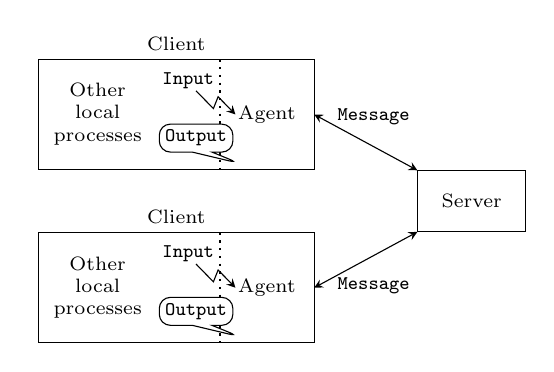
\begin{tikzpicture}[%
  >=stealth,
  msg/.style={font=\scriptsize\ttfamily},
  every node/.style={font=\scriptsize},
  client/.pic={
    \coordinate (-west) at (3.5,-0.7);
    \draw (0,0) -- (3.5,0) -- (3.5,-1.4) -- (0,-1.4) -- cycle;
    \draw[dotted,thick] (2.3,0) -- (2.3, -1.4);
    \node at (1.75,0.2) {Client};
    \node (op) at (0.75,-0.7) {
      \begin{tabular}{c}
        Other\\local\\processes        
      \end{tabular}
    };
    \node (a) at (2.9,-0.7) {
      Agent
    };
    \begin{scope}[shift={(2.5,-0.7)}, yscale=1.5]
      \draw[->] (-0.5,0.2) node[above=-1mm,shift={(-0.1,0)},msg] {Input} -- (-0.28,0.05) -- (-0.22,0.15) -- (0,0);
    \end{scope}
    \begin{scope}[shift={(2.5,-1.2)}]
      \node[inner sep=0.75mm, draw, fill=white, rectangle callout, rounded corners, callout absolute pointer={(0.05,-0.12)}, msg] (out) at (-0.5,0.2) {Output};
      % 
    \end{scope}
  }]
  \pic (c1) at (0,0) {client};
  \pic (c2) at (0,2.2) {client};
  \node[draw,inner sep=3mm] (s) at ($(c1-west)!0.5!(c2-west) + (2,0)$) {Server};
  \draw[<->] (c1-west) -- node[msg,below,shift={(0.1,-0.1)}] {Message} (s.south west);
  \draw[<->] (c2-west) -- node[msg,above,shift={(0.1,0.1)}] {Message} (s.north west);
\end{tikzpicture}


  \caption{Architecture of a lock service application. Boxes represent separate
    physical nodes, while dotted lines separate processes running on
    the same node.  Each client node runs an Agent process that
    exchanges input and output with other local processes.  The Agent
    also exchanges network messages with the Server.}

\label{fig:lock-service-architecture}
\end{figure}

To provide this API, the lock service consists of a central lock Server
node, and a lock Agent that runs on every client node, as illustrated in
\cref{fig:lock-service-architecture}.
%
That is, each client node runs a lock Agent along with other client
processes that access the API through the Agent.
%
Each lock Agent communicates over the network with the central lock server.
%
The Agent requests and releases the lock with the \LockMsg and \UnlockMsg
network messages, and the server sends a \GrantMsg network message to
notify an Agent when it has received the lock.
%
% Note that, while the network may suffer disruptions, the input/output
% messages \LockIO, \UnlockIO, and \GrantIO are sent within a node and are
% delivered reliably and in order.

% We first overview building and verifying the system in a reliable
% network where machines never crash and packets may be reordered, but
% are never dropped or duplicated.  Then we show how a verified
% system transformer can be used, \emph{without any
%   additional proof effort}, to obtain a correctness proof for this
% system in a more adversarial network where packets are dropped and
% duplicated.  More details about these network semantics are discussed
% in \cref{sec:verdi:nwsem}.

\begin{figure}[p]
\begin{footnotesize}
\begin{Verbatim}[commandchars=\\\{\},codes={\catcode`\$=3\catcode`\^=7\catcode`\_=8}]
\PY{c}{(*}\PY{c}{ 1 \PYZhy{} node identifiers }\PY{c}{*)}
\PY{n+nc}{Name} \PY{o}{:=} \PY{n+nc}{Server} \PY{o}{|} \PY{n+nc}{Agent}\PY{o}{(}\PY{k+kt}{int}\PY{o}{)}

\PY{c}{(*}\PY{c}{ 2 \PYZhy{} API, also known as external IO }\PY{c}{*)}
\PY{n+nc}{Inp} \PY{o}{:=} \PY{n+nc}{Lock} \PY{o}{|} \PY{n+nc}{Unlock}
\PY{n+nc}{Out} \PY{o}{:=} \PY{n+nc}{Grant}
\PY{c}{(*}\PY{c}{ 2 \PYZhy{} network messages }\PY{c}{*)}
\PY{n+nc}{Msg} \PY{o}{:=} \PY{n+nc}{LockMsg} \PY{o}{|} \PY{n+nc}{UnlockMsg} \PY{o}{|} \PY{n+nc}{GrantMsg}

\PY{c}{(*}\PY{c}{ 3 \PYZhy{} state }\PY{c}{*)}
\PY{n+nc}{State} \PY{o}{(}\PY{n}{n}\PY{o}{:} \PY{n+nc}{Name}\PY{o}{)} \PY{o}{:=}
  \PY{k}{match} \PY{n}{n} \PY{k}{with}
    \PY{o}{|} \PY{n+nc}{Server} \PY{o}{=\PYZgt{}} \PY{k+kt}{list} \PY{n+nc}{Name} \PY{c}{(*}\PY{c}{ head = agent holding lock      }\PY{c}{*)}
                          \PY{c}{(*}\PY{c}{ tail = agents waiting for lock }\PY{c}{*)}
    \PY{o}{|} \PY{n+nc}{Agent} \PY{n}{n} \PY{o}{=\PYZgt{}} \PY{k+kt}{bool}     \PY{c}{(*}\PY{c}{ true iff this agent holds lock }\PY{c}{*)}

\PY{n+nc}{InitState} \PY{o}{(}\PY{n}{n}\PY{o}{:} \PY{n+nc}{Name}\PY{o}{)} \PY{o}{:} \PY{n+nc}{State} \PY{n}{n} \PY{o}{:=}
  \PY{k}{match} \PY{n}{n} \PY{k}{with}
    \PY{o}{|} \PY{n+nc}{Server} \PY{o}{=\PYZgt{}} \PY{n+nb+bp}{[]}
    \PY{o}{|} \PY{n+nc}{Agent} \PY{n}{n} \PY{o}{=\PYZgt{}} \PY{n+nb+bp}{false}

\PY{c}{(*}\PY{c}{ 4 \PYZhy{} handler for external input }\PY{c}{*)}
\PY{n+nc}{HandleInp} \PY{o}{(}\PY{n}{n}\PY{o}{:} \PY{n+nc}{Name}\PY{o}{)} \PY{o}{(}\PY{n}{s}\PY{o}{:} \PY{n+nc}{State} \PY{n}{n}\PY{o}{)} \PY{o}{(}\PY{n}{inp}\PY{o}{:} \PY{n+nc}{Inp}\PY{o}{)} \PY{o}{:=}
  \PY{k}{match} \PY{n}{n} \PY{k}{with}
    \PY{o}{|} \PY{n+nc}{Server} \PY{o}{=\PYZgt{}} \PY{n}{nop}   \PY{c}{(*}\PY{c}{ server performs no external IO }\PY{c}{*)}
    \PY{o}{|} \PY{n+nc}{Agent} \PY{n}{n} \PY{o}{=\PYZgt{}}
      \PY{k}{match} \PY{n}{inp} \PY{k}{with}
        \PY{o}{|} \PY{n+nc}{Lock} \PY{o}{=\PYZgt{}}                     \PY{c}{(*}\PY{c}{ client requests lock   }\PY{c}{*)}
          \PY{n}{send} \PY{o}{(}\PY{n+nc}{Server}\PY{o}{,} \PY{n+nc}{LockMsg}\PY{o}{)}      \PY{c}{(*}\PY{c}{ forward to Server      }\PY{c}{*)}
        \PY{o}{|} \PY{n+nc}{Unlock} \PY{o}{=\PYZgt{}}                   \PY{c}{(*}\PY{c}{ client requests unlock }\PY{c}{*)}
          \PY{k}{if} \PY{n}{s} \PY{o}{=}\PY{o}{=} \PY{n+nb+bp}{true} \PY{k}{then} \PY{o}{(}         \PY{c}{(*}\PY{c}{ if lock held           }\PY{c}{*)}
            \PY{n}{s} \PY{o}{:=} \PY{n+nb+bp}{false}\PY{o}{;;}              \PY{c}{(*}\PY{c}{ update state           }\PY{c}{*)}
            \PY{n}{send} \PY{o}{(}\PY{n+nc}{Server}\PY{o}{,} \PY{n+nc}{UnlockMsg}\PY{o}{)}\PY{o}{)} \PY{c}{(*}\PY{c}{ tell Server lock freed }\PY{c}{*)}

\PY{c}{(*}\PY{c}{ 4 \PYZhy{} handler for network messages }\PY{c}{*)}
\PY{n+nc}{HandleMsg} \PY{o}{(}\PY{n}{n}\PY{o}{:} \PY{n+nc}{Name}\PY{o}{)} \PY{o}{(}\PY{n}{s}\PY{o}{:} \PY{n+nc}{State} \PY{n}{n}\PY{o}{)} \PY{o}{(}\PY{n}{src}\PY{o}{:} \PY{n+nc}{Name}\PY{o}{)} \PY{o}{(}\PY{n}{msg}\PY{o}{:} \PY{n+nc}{Msg}\PY{o}{)} \PY{o}{:=}
  \PY{k}{match} \PY{n}{n} \PY{k}{with}
    \PY{o}{|} \PY{n+nc}{Server} \PY{o}{=\PYZgt{}}
      \PY{k}{match} \PY{n}{msg} \PY{k}{with}
        \PY{o}{|} \PY{n+nc}{LockMsg} \PY{o}{=\PYZgt{}}
          \PY{c}{(*}\PY{c}{ if lock not held, immediately grant }\PY{c}{*)}
          \PY{k}{if} \PY{n}{s} \PY{o}{=}\PY{o}{=} \PY{n+nb+bp}{[]} \PY{k}{then} \PY{n}{send} \PY{o}{(}\PY{n}{src}\PY{o}{,} \PY{n+nc}{GrantMsg}\PY{o}{)}\PY{o}{;;}
          \PY{c}{(*}\PY{c}{ add requestor to end of queue }\PY{c}{*)}
          \PY{n}{s} \PY{o}{:=} \PY{n}{s} \PY{o}{+}\PY{o}{+} \PY{o}{[}\PY{n}{src}\PY{o}{]}
        \PY{o}{|} \PY{n+nc}{UnlockMsg} \PY{o}{=\PYZgt{}}
          \PY{c}{(*}\PY{c}{ head of queue no longer holds lock }\PY{c}{*)}
          \PY{n}{s} \PY{o}{:=} \PY{n}{tail} \PY{n}{s}\PY{o}{;;}
          \PY{c}{(*}\PY{c}{ grant lock to next waiting agent, if any }\PY{c}{*)}
          \PY{k}{if} \PY{n}{s} \PY{o}{!=} \PY{n+nb+bp}{[]} \PY{k}{then} \PY{n}{send} \PY{o}{(}\PY{n}{head} \PY{n}{s}\PY{o}{,} \PY{n+nc}{GrantMsg}\PY{o}{)}
        \PY{o}{|} \PY{o}{\PYZus{}} \PY{o}{=\PYZgt{}} \PY{n}{nop} \PY{c}{(*}\PY{c}{ never happens }\PY{c}{*)}
    \PY{o}{|} \PY{n+nc}{Agent} \PY{n}{n} \PY{o}{=\PYZgt{}}
      \PY{k}{match} \PY{n}{msg} \PY{k}{with}
        \PY{o}{|} \PY{n+nc}{GrantMsg} \PY{o}{=\PYZgt{}}      \PY{c}{(*}\PY{c}{ lock acquired    }\PY{c}{*)}
          \PY{n}{s} \PY{o}{:=} \PY{n+nb+bp}{true}\PY{o}{;;}      \PY{c}{(*}\PY{c}{ update state     }\PY{c}{*)}
          \PY{n}{output} \PY{n+nc}{Grant}     \PY{c}{(*}\PY{c}{ notify listeners }\PY{c}{*)}
        \PY{o}{|} \PY{o}{\PYZus{}} \PY{o}{=\PYZgt{}} \PY{n}{nop}         \PY{c}{(*}\PY{c}{ never happens    }\PY{c}{*)}
\end{Verbatim}

\end{footnotesize}

\caption{A simple lock service application implemented in \Verdi, under the
  assumption of a reliable network.  \Verdi extracts these definitions into
  OCaml and links the resulting code with a runtime to send and receive
  messages over the network.}
\label{fig:lock-service-code}
\end{figure}

\subsection{Specification}

A \Verdi programmer specifies the correct behavior of their system in
terms of \textit{traces}, the sequences of external input and output
generated by nodes in the system.
%
For the lock service application, correctness requires mutual exclusion: no
two distinct nodes should ever simultaneously hold the lock.
%
This mutual exclusion property can be expressed as a predicate over traces:
%
\[ \begin{array}{l}
  \relax\property{mutex}(\tau) \coloneq \NL
  \iV \tau \;=\; \tau_1 \appop
             \tevent{n_1}{\GrantIO} \appop
             \tau_2 \appop
             \tevent{n_2}{\GrantIO} \appop
             \tau_3 \NL
  \iV \rightarrow
    \tevent{n_1}{\UnlockIO} \in \tau_2
\end{array} \]
%
To hold on trace $\tau$, the $\property{mutex}$ predicate requires that
whenever \GrantIO is output on node $n_1$ and then later \GrantIO is output
on node $n_2$, there must first be an intervening \UnlockIO input from
$n_1$ releasing the lock.

A system implementation satisfies specification $\tracespec$ in a
particular network semantics if for all traces $\tau$ the system can
produce under that semantics, $\tracespec$ holds on $\tau$.  For the
example lock service application, an implementation satisfies
\property{mutex} in a given semantics if \property{mutex} holds on all the
traces produced under that semantics.


%% {\smaller\setlength{\arraycolsep}{.5\arraycolsep}%
%% \begin{eqnarray*}
%%   \property{mutex}(\tau)\ & \mathtt{:=} & \property{mutex'}(\tau, \mathtt{None})
%%   \\
%%   \property{mutex'}([], \mathtt{None}) & \mathtt{:=} & \mathtt{true}
%%   \\
%%   \property{mutex'}([], n) & \mathtt{:=} & \mathtt{true}
%%   \\
%%   \property{mutex'}(\traceelt{n', \GrantIO} :: \tau', \mathtt{None})
%%   & \mathtt{:=} &  \property{mutex'}(\tau', n')
%%   \\
%%   \property{mutex'}(\traceelt{n', \GrantIO} :: \tau', n)
%%   & \mathtt{:=} & \mathtt{false} % \quad \text{ if } n \ne \mathtt{None}
%%   \\
%%   \property{mutex'}(\traceelt{n, \UnlockIO} :: \tau', n)
%%   & \mathtt{:=} & \property{mutex'}(\tau', \mathtt{None})
%%   \\
%%   \property{mutex'}(\traceelt{n', \UnlockIO} :: \tau', n)
%%   & \mathtt{:=}
%%   &  \property{mutex'}(\tau', n)  \quad \text{ if } n' \ne n
%%   \\
%%   \property{mutex'}(\traceelt{n', \LockIO} :: \tau', n)
%%   & \mathtt{:=} & \property{mutex'}(\tau', n)
%% \end{eqnarray*}%
%% }%

\subsection{Implementation}

Figure~\ref{fig:lock-service-code} shows the definitions a programmer
provides to implement the lock service application in \Verdi.
%
(1) \Name lists the names of nodes in the system.
%
In the lock service application, there is a single Server node and an
arbitrary number of Agents.
%
(2) \Input and \Output define the API of the lock service --- the external
input and output exchanged between an Agent and other local processes on
its node.
%
\Message defines network messages exchanged between Agents and the central
Server.
%--- this is an implementation detail of the lock service.
%
(3) \VerdiState defines the state maintained at each node.
Node state is defined as a dependent type where a node's name determines
the data maintained locally at that node.
%
In the lock service, the Server maintains a queue of Agent nodes,
initially empty, where the head of the queue is the Agent currently
holding the lock and the rest of the queue represents the Agents which
are waiting to acquire the lock.
%
Each Agent maintains a boolean, initially false, which is true exactly when
that Agent holds the lock.
%
(4) The handler functions \HandleInput and \HandleMessage define how
nodes respond to external input and to network messages.

This implementation assumes a reliable network where machines never crash
and packets may be reordered but are not dropped or duplicated.
%
These assumptions reduce the programmer's effort in both implementing the
application and proving it correct.
%
\Cref{sec:verdi:failures-locksrv} shows how \Verdi can automatically transform
the lock service application into a version that tolerates faults.

When the system runs, each node listens for events and responds by running
the appropriate handler: \HandleInput for external input and \HandleMessage
for network messages.
%
% External input
%
When an Agent receives an external input that requests to acquire or
release the lock, it forwards the request to the Server; in the \UnlockIO
case, it first checks to ensure that the lock is actually held, and it
resets its local state to \mytt{false}.
Because the network is assumed to be reliable, no acknowledgment
of the release is needed from the Server.
%
%% This feels redundant to Mike.
% Note that the Server does not act on any external input or generate
% any external output.
%
% Network messages
%
When the Server receives a \LockMsg network message, if the lock is not
held, the server immediately grants the lock, and always adds the
requesting Agent to the end of the queue of nodes.
%
When the Server receives an \UnlockMsg message, it removes a node from the
head of its queue of Agents and grants the lock to the next Agent in the
queue, if any.
%
When an Agent receives a \GrantMsg message, it produces external output
(\GrantIO) to inform other processes running on its node that the lock is
held.

The application will be deployed on some network, and \emph{network
semantics} capture assumptions about the network's behavior.
%
For this example, we assume a semantics encoding a reliable network.
%
In a reliable network, each step of execution either (1) picks an arbitrary
node and delivers an arbitrary external input, runs that node's input
handler, and updates the state, or (2) picks a message in the network, runs
the recipient's message handler, and updates the state.

Figure~\ref{fig:lock-service-diagram} shows an execution of the lock
service application with two agents.
%
Agents $A_1$ and $A_2$ both try to acquire the lock. The service first
grants the lock to $A_1$.
%
Once $A_1$ releases the lock, the service grants it to $A_2$.
%
Note that, because our network semantics does not assume messages are
delivered in the same order in which they were sent, there is a potential
race condition: an agent can attempt to re-acquire the lock before the
server has processed its previous release.
%
In that case, the server simply (and correctly) adds the sender to the
queue again.
%
Using \Verdi, the lock service is guaranteed to behave correctly even
in such corner cases.
\begin{figure}[t]
  \centering
  % \includegraphics[width=\columnwidth]{lock}
  \usetikzlibrary{backgrounds}
\usetikzlibrary{calc}
\usetikzlibrary{positioning}
\usetikzlibrary{shapes.callouts}

\def\cOneX{0}
\def\sX{2}
\def\cTwoX{4}
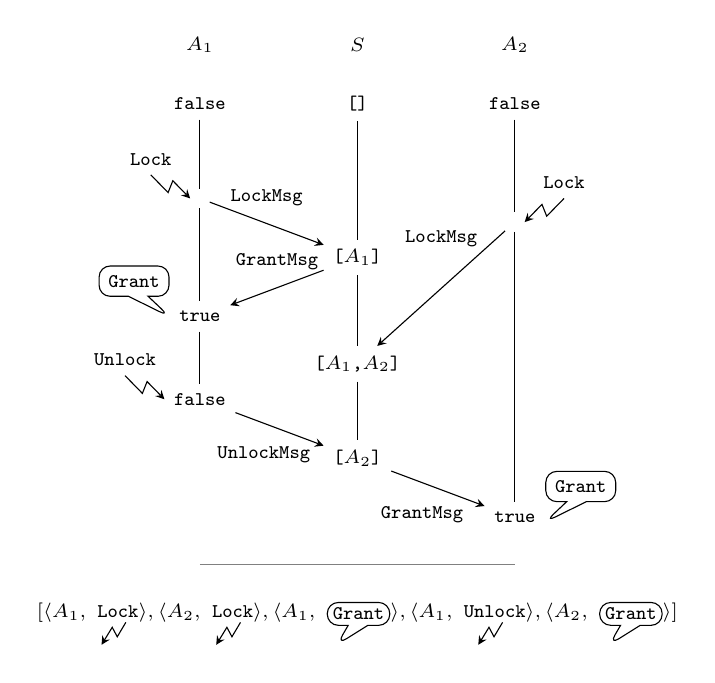
\begin{tikzpicture}[yscale=1.5,
  >=stealth,
  every node/.style={font=\scriptsize},
  state/.style={font=\scriptsize\bf\ttfamily},
  msg/.style={font=\scriptsize\ttfamily}
  ]
  \node (c1) at (\cOneX,0) {$A_1$};
  \node (s) at (\sX,0) {$S$};
  \node (c2) at (\cTwoX,0) {$A_2$};

  % \draw[->] (7, -1) -- node[above,rotate=90] {time} (7, -10);

  \node[state] (c1-init) at (\cOneX,-0.5) {false};
  \node[state] (s-init) at (\sX,-0.5) {[]};
  \node[state] (c2-init) at (\cTwoX,-0.5) {false};


  \def\verdiInputL#1#2{%
    {%
      \def\beginning{($#1 + (-0.5,0.2)$)}%
      \def\cOne{($#1 + (-0.28,0.05)$)}%
      \def\cTwo{($#1 + (-0.22,0.15)$)}%

      % \draw[gray] \beginning -- \cOne;%
      % \fill[gray] \cOne circle (0.2mm);%
      % \draw[gray] \cTwo -- #1;%
      % \fill[gray] \cTwo circle (0.2mm);%
      \draw[->] \beginning node[above,msg] {#2} -- \cOne -- \cTwo -- #1 ;%
    }
  }

  \def\verdiInputR#1#2{%
    {%
      \def\beginning{($#1 + (0.5,0.2)$)}%
      \def\cOne{($#1 + (0.28,0.05)$)}%
      \def\cTwo{($#1 + (0.22,0.15)$)}%

      % \draw[gray] \beginning -- \cOne;%
      % \fill[gray] \cOne circle (0.2mm);%
      % \draw[gray] \cTwo -- #1;%
      % \fill[gray] \cTwo circle (0.2mm);%
      \draw[->] \beginning node[above,msg] {#2} -- \cOne -- \cTwo -- #1 ;%
    }
  }

  \def\verdiOutputL#1#2{%
    {%
      \node[msg, draw, rectangle callout, rounded corners, callout absolute pointer={#1}, anchor=east,] at ($#1 + (0,0.3)$) {#2};
    }
  }
  \def\verdiOutputR#1#2{%
    {%
      \node[msg, draw, rectangle callout, rounded corners, callout absolute pointer={#1}, anchor=west,] at ($#1 + (0,0.3)$) {#2};
    }
  }

  \def\verdiMsgAbove#1#2#3{%
    \draw[->] #1 -- node[msg,above,yshift=1mm] {#3} #2;%
  }

  \def\verdiMsgBelow#1#2#3{%
    \draw[->] #1 -- node[msg,below,shift={(-2mm,-1mm)}] {#3} #2;%
  }

  \node[state] (c1-send-lock) at (\cOneX, -1.3) {};
  \verdiInputL{(c1-send-lock.west)}{\LockIO}

  \node[state] (s-recv-c1-lock) at (\sX, -1.8) {[$A_1$]};
  \verdiMsgAbove{(c1-send-lock)}{(s-recv-c1-lock)}{\LockMsg}
  \node[state] (c1-recv-grant) at (\cOneX, -2.3) {true};
  \verdiMsgAbove{(s-recv-c1-lock)}{(c1-recv-grant)}{\GrantMsg}
  \verdiOutputL{(c1-recv-grant.west)}{\GrantIO}

  \node[state] (c2-send-lock) at (\cTwoX, -1.5) {};
  \verdiInputR{(c2-send-lock.east)}{\LockIO}
  \node[state] (s-recv-c2-lock) at (\sX, -2.7) {[$A_1$,$A_2$]};
  \draw[->] (c2-send-lock) -- node[msg,above,yshift=4mm] {\LockMsg} (s-recv-c2-lock);%


  \node[state] (c1-send-unlock) at (\cOneX, -3) {false};
  \verdiInputL{(c1-send-unlock.west)}{\UnlockIO}

  \node[state] (s-recv-c1-unlock) at (\sX, -3.5) {[$A_2$]};
  \verdiMsgBelow{(c1-send-unlock)}{(s-recv-c1-unlock)}{\UnlockMsg}

  \node[state] (c2-recv-grant) at (\cTwoX, -4) {true};
  \verdiMsgBelow{(s-recv-c1-unlock)}{(c2-recv-grant)}{\GrantMsg}
  \verdiOutputR{($(c2-recv-grant.east) !.3! (c2-recv-grant.south east)$)}{\GrantIO}

  \draw (c1-init) -- (c1-send-lock) -- (c1-recv-grant) -- (c1-send-unlock);
  \draw (s-init) -- (s-recv-c1-lock) -- (s-recv-c2-lock) -- (s-recv-c1-unlock);
  \draw (c2-init) -- (c2-send-lock) -- (c2-recv-grant);

  \begin{scope}[shift={(-1,-4.4)},
    every node/.style={font=\scriptsize},
    outp/.style={inner sep=0.7mm,draw,rectangle callout, rounded corners, callout relative pointer={(235:3mm)}}]
    \draw[gray] (1,0) -- (5,0);
    \def\verdiInputR#1#2{%
      {%
        \begin{scope}[rotate=25]
          \def\beginning{($#1 + (0.5,0.2)$)}%
          \def\cOne{($#1 + (0.324,0.08)$)}%
          \def\cTwo{($#1 + (0.3168,0.216)$)}%
          \def\ending{($#1 + (0.10,0.072)$)}%

          % \draw[gray] \beginning -- \cOne;%
          % \fill[gray] \cOne circle (0.2mm);%
          % \draw[gray] \cTwo -- #1;%
          % \fill[gray] \cTwo circle (0.2mm);%
          \draw[->] \beginning node[inner sep=0mm,above,msg,xshift=-1mm,yshift=0.5mm] {#2} -- \cOne -- \cTwo -- \ending ;%
        \end{scope}
      }
    }

    \node (trace) at (3,-0.5) {$[\tevent{A_1}{\tikz[baseline=4.5mm]{\verdiInputR{(0,0)}{\LockIO}}},%
      \tevent{A_2}{\tikz[baseline=4.5mm]{\verdiInputR{(0,0)}{\LockIO}}},%
      \tevent{A_1}{\tikz[baseline=-0.5mm]{\draw node[inner sep=0.7mm,draw,rectangle callout, rounded corners, callout relative pointer={(235:3mm)}] {\GrantIO}}},%
      \tevent{A_1}{\tikz[baseline=4.5mm]{\verdiInputR{(0,0)}{\UnlockIO}}},%
      \tevent{A_2}{\tikz[baseline=-0.5mm]{\draw node[inner sep=0.7mm,draw,rectangle callout, rounded corners, callout relative pointer={(235:3mm)}] {\GrantIO}}}]$};
    %\node[below of=trace,node distance=2mm] (empty-filler)  {};
  \end{scope}

  % \node[state] (c2-send-unlock) at (\cTwoX, -5) {false};
  % \verdiInputR{(c2-send-unlock.east)}{\UnlockIO}
  % \node[state] (s-recv-c2-unlock) at (\sX, -5.5) {[]};
  % \verdiMsgAbove{(c2-send-unlock)}{(s-recv-c2-unlock)}{\UnlockMsg}
\end{tikzpicture}%these comments prevent extra whitespace
%

  \caption{The behavior of the lock service application, with one
    server~$S$ and two agents~$A_1$ and $A_2$.
    %
    Each agent starts with the state \mytt{false}, and the server starts
    with an empty queue.
    %
    Time flows downward.
    %
    In response to external input (drawn with lightning-bolt arrows) and
    network messages, the nodes exchange messages and update local state.
    %
    External output is shown as speech bubbles.
    %
    The trace of this execution is shown at the bottom; note that only
  externally-visible events (external input and output) appear in the trace.}

\label{fig:lock-service-diagram}
\end{figure}

\subsection{Verifying the Lock Service Application}

We briefly outline the proof of the \property{mutex} property for the lock
service application in the reliable network environment~(\ie, no machine
crashes nor packet loss/duplication).
%
The proof that \property{mutex} holds on all traces of the lock service
application consists of three high-level steps: (1) prove an invariant
about the reachable node and network states of the lock service
application, (2) relate these reachable states to the producible traces,
and (3) show that the previous two steps imply \property{mutex} holds on all
producible traces.

The first step proves that all reachable system states satisfy the
$\mutexstate$ property:
%
 \[ \begin{array}{l}
  \mutexstate(\Sigma,\ P)\ \coloneq \NL
  \iV  \forall\ n\ m,\ n \ne m \to
       \neg \property{hasLock}(\Sigma,\ n) \lor
       \neg \property{hasLock}(\Sigma,\ m) \BR
  \property{hasLock}(\Sigma,\ n)\ \coloneq \NL
  \iV  \Sigma(\mbox{Agent}(n)) = \<true>
\end{array} \]
%
The function $\Sigma$ maps node names to their state, and $P$ is the set of
in-flight packets. The property $\mutexstate$ ensures
that at most one Agent node holds the lock at a time.

A programmer can verify the $\mutexstate$ property by proving
an \textit{inductive state invariant}.
%
A property $\phi$ is an inductive invariant if both
%
(1) it holds in the initial state, $(\Sigma_0,\ \emptyset)$, where
$\Sigma_0$ maps each node to its initial state and $\emptyset$ represents
the initial, empty network, and also
%
(2) whenever it holds in some state, $(\Sigma,\ P)$, and $(\Sigma,\ P)$
can step to $(\Sigma',\ P')$, then it holds in $(\Sigma',\ P')$.

One inductive state invariant for \mutexstate is:
%
\begin{align*}
         & \left(\forall\ n,\, \property{hasLock}(\Sigma,\ n) \to \property{atHead}(\Sigma,\ n)\right)\\
  \wedge & \left(\forall\ p\in P,\ p.\<body> = \GrantMsg \to \property{grantee}(\Sigma,\ p.\<dest>)\right)\\
  \wedge & \left(\forall\ p\in P,\ p.\<body> = \UnlockMsg \to \property{grantee}(\Sigma,\ p.\<source>)\right)\\
  \wedge & ~\property{at\_most\_one}\ \{\GrantMsg,\ \UnlockMsg\}\ P
\end{align*}%
 where%
\begin{align*}
  \property{atHead}(\Sigma,\ n) \quad \coloneq & \quad \exists\ t,\ \Sigma(\mbox{Server}) = n :: t \\
  \property{grantee}(\Sigma,\ n) \quad \coloneq & \quad \property{atHead}(\Sigma,\ n) \wedge \neg \property{hasLock}(\Sigma,\ n).
\end{align*}%
%
The first conjunct above ensures that the Server and Agents agree on who
holds the lock.
%
The second and third conjuncts state that \GrantMsg is never
sent to an agent that already holds the lock, and that \UnlockMsg
is never sent from an agent that still holds the lock.
%
Finally, the last conjunct states that there is at most one in-flight
message in the set $\{\GrantMsg, \UnlockMsg\}$; this is necessary to
ensure that neither of the previous two conjuncts is violated when a
message is delivered.
%
We proved in \Coq that this invariant is inductive and that it implies
$\mutexstate$; the proof is approximately 500 lines long.


The second step of the proof relates reachable states to the traces a system
can produce:
%
\[ \begin{array}{l}
  \property{trace\_state\_agreement}(\tau,\ \Sigma)\ \coloneq \NL
  \iV  \forall\ n,\ \property{lastGrant}(\tau,\ n)
       \leftrightarrow \property{hasLock}(\Sigma,\ n) \BR
%
  \property{lastGrant}(\tau, n)\ \coloneq \NL
  \iV  \tau = \tau_1 \appop
              \tevent{n}{\GrantIO} \consop
              \tau_2 \wedge
              \forall\ m,\ \tevent{m}{\UnlockIO} \not\in \tau_2 \BR
\end{array} \]
%
This property requires that whenever a \GrantIO output appears in
the trace without a corresponding \UnlockIO input, that agent's flag is
true (and vice versa).
%
The proof of this property is by induction on the possible behavior of
the network.

The third step of the proof shows that together,
\mutexstate and \property{trace\_state\_agreement} imply
that \property{mutex} holds on all traces of the lock service
application under the reliable semantics. This result follows
from the definitions of $\property{mutex}$, $\mutexstate$,
and $\property{trace\_state\_agreement}$.

\subsection{Verified System Transformers}
\label{sec:verdi:failures-locksrv}

We have proved the \property{mutex} property for a reliable environment
where the network does not drop or duplicate packets and the server does
not crash.
%
Assuming such a reliable environment simplifies the proof by allowing the
programmer to consider fewer cases.
%
To transfer the property into an unreliable environment with network and
machine failures, a programmer uses \Verdi's verified system transformers.
%
As illustrated by Figure~\ref{fig:verdi-components} part~\numcircled{4},
after verifying a distributed system in one network semantics, a programmer
can apply a verified system transformer to produce another version of their
system which provides analogous guarantees in another network semantics.

In general, there are two types of transformers in \Verdi:
\textit{transmission transformers} that handle network faults like packet
duplication and drops and \textit{replication transformers} that handle
node crashes.
%
Below we describe an example transmission transformer for the lock
service application and briefly overview replication transformers,
deferring details to \cref{sec:verdi:casestudy-raft}.

\para{Tolerating network faults} \cref{fig:lock-service-code}'s
implementation of the lock service application will \emph{not} function
correctly in a network where messages can be duplicated.
%
If an \UnlockMsg message is duplicated but the agent reacquires the lock
before the second copy is delivered, the server will misinterpret the
duplicated \UnlockMsg message as releasing the second lock acquisition.

Realistically, most developers would not run into this issue, as
correct TCP implementations reject duplicate transmissions. However,
some distributed systems need to handle deduplication and
retransmission at a higher level, or choose not to trust the
guarantees provided by unverified TCP implementations.

As another option, a programmer could rewrite the lock service---for
instance, by including a unique identifier with
every \GrantMsg and \UnlockMsg message to ensure that they are
properly paired.
%
The developer would then need to re-prove system correctness for this
slightly different system in the semantics that models packet-duplicating
networks.
%
This would require finding a new inductive invariant and writing another
proof.

%
\Verdi allows developers to skip these steps. \Verdi provides a system
transformer that adds sequence numbers to every outgoing packet and
ignores packets with sequence numbers that have already been seen.
%
Applying this transformer to the lock service yields both a new system
\textit{and a proof} that the new system preserves the \property{mutex}
property even when packets are duplicated by the underlying network.
%
Section~\ref{sec:verdi:libraries} further details this transformer.

More generally, \Verdi decouples the verification of application-level
guarantees from the implementation and verification of fault-tolerance
mechanisms.
%
\Verdi provides a collection of verified system transformers which allow
the developer to transfer guarantees about a system in one network
semantics to analogous guarantees about a transformed version of the
system in another network semantics.
%
This allows a programmer to build and verify their system against an
idealized semantics and use a verified system transformer to obtain a
version of the system that provably tolerates more realistic faults while
guaranteeing end-to-end system correctness properties.

% The current lock service application cannot tolerate server crashes.
\para{Tolerating machine crashes}
\Verdi also provides verified system transformers to tolerate
machine crashes via replication.  Such replication transformers generally
create multiple copies of a node in order tolerate machine crashes.
%
This changes the number of nodes when transforming a system, which we
discuss further in \cref{sec:verdi:casestudy-raft}.
%
(By contrast, transmission transformers like the one described above
generally preserve the number of nodes and the relationships between them
when transforming a distributed system.)


\subsection{Running the Lock Service Application}

Now we have a formally verified lock service, written in \Coq,
that tolerates message duplication faults.
%
To obtain an executable for deployment, a \Verdi programmer invokes \Coq's
built-in extraction mechanism to generate OCaml code from the \Coq
implementation, compile it with the OCaml compiler, and link it with a
\Verdi shim.
%
The shim is written in OCaml; it implements network primitives~(e.g.,
packet send/receive) and an event loop that invokes the appropriate event
handler for incoming network packets, IO, or other events.

\subsection{Summary}

We have demonstrated how to use \Verdi to establish a strong guarantee of
the \property{mutex} property for the lock service application running in a
realistic environment.
%
Specifically, a programmer first specifies, implements, and verifies an
application assuming a reliable environment.
%
The programmer then applies system transformers to obtain a version of
their application that handles faults in a provably correct way.

\Verdi's trusted computing base includes the following components: the
specifications of verified applications, the assumption that \Verdi's
network semantics match the physical network, the \Verdi shim, \Coq's
proof checker and OCaml code extractor, and the OCaml compiler and
runtime.

\Verdi currently supports verifying safety properties, but not liveness
properties, and none of \Verdi's network semantics currently capture
Byzantine fault models.
%
We believe that \Verdi could be extended to support these features:
liveness properties could be verified by supporting infinite traces and
adding fairness hypotheses as axioms as in TLA~\cite{lamport:tla}, while
Byzantine fault models can be supported by adding more non-determinism in
the network semantics.

%%  LocalWords:  implementing-in-verdi init initState getState putState.
%%  LocalWords:  handleNet handleIO e.g. handleLocalInput enqueues boolean
%%  LocalWords:  mutex nwsem monadic Haskell-like dest VST mutex' n' pbj
%%  LocalWords:  locksrv lastGrant hasLock atHead casestudy

\section{Network Semantics}\label{sec:verdi:nwsem}

The correctness of a distributed system relies on assumptions about its
environment.
%
For example, one distributed system may assume a reliable network, while
others may be designed to tolerate packet reordering, loss, or
duplication.
%
To enable programmers to reason about the correctness of distributed
systems in the appropriate environment model, \Verdi provides a spectrum of
\emph{network semantics} that encode possible system behaviors using
small-step style derivation rules.

This section presents the spectrum of network semantics that \Verdi
provides, ranging from single-node systems that do not
rely on the network, through models of increasingly unreliable packet
delivery (reordering, drops, and duplication), and culminating with a
model that permits arbitrary node crashes under various recovery
assumptions.
%
Each of these semantics is useful for reasoning about different types of
systems.
%
For example, the properties of single-node systems can be extended
to handle node failures using protocols like
Raft, while packet duplication semantics is useful for verifying
packet delivery even in the face of reconnection, something that
raw TCP does not support.

%% To add an additional fault model to \Verdi, a programmer provides the
%% derivation rules for their network semantics, which often simply requires
%% modifying or adding inference rules to one of the semantics described
%% below.
%% %
%% As discussed later in Section~\ref{sec:verdi:libraries}, formalizing different
%% fault models as distinct network semantics played an enabling role in
%% verified system transformers, the key to modular verification in \Verdi.

\begin{figure}[t]
  \centering

  \begin{footnotesize} \begin{spacing}{1.5} \[
    \inferrule*[right=\textsc{Input}]{
      \fHinp(\sigma,\ i) = (\sigma',\ o)
    }{
      (\sigma,\ T) \fsmstep (\sigma',\ T \appop \traceelt{i,\ o})
    }
  \] \end{spacing} \end{footnotesize}

  \caption{Single-node semantics.
  %
  The derivation rule above encodes possible behaviors of a single-node
  system that does not rely on the network.
  %
  When the node is in state $\sigma$ with input/output trace $T$, it may
  receive an arbitrary input $i$, and respond by running its input handler
  $\fHinp(\sigma,\ i)$, which generates both the next state $\sigma'$ and a list of
  outputs $o$.
  %
  The \textsc{Input} rule relates the two states of the world $(\sigma,\ T) \fsmstep
  (\sigma',\ T \appop \traceelt{i,\ o})$ to reflect that the node has updated
  its state to $\sigma'$ and sent outputs $o$ in response to input $i$.
  %
  Verifying properties of such single-node systems (\ie state machines) is
useful when they are replicated over a network to provide fault tolerance.}

\label{fig:state-machine-semantics}
\end{figure}

In Verdi, network semantics are defined as step relations on a ``state of
the world''.
%
The state of the world differs among network semantics, but always includes
a trace of the system's external input and output.
%
For example, many semantics include a bag of in-flight packets
that have been sent by nodes in the system but have not yet been delivered
to their destinations.
%
Each network semantics is parameterized by system-specific data types and
handler functions.
%
Below we detail several of the network semantics \Verdi currently provides.

\paragraph{Single-node semantics} We begin with a simple semantics for
single-node systems that do not use the network, \ie state machines.
%
This semantics is useful for proving properties of single-node systems;
these can be extended, using a verified system transformer based on Raft,
to provide fault tolerance.
%
The single-node semantics, shown in \cref{fig:state-machine-semantics},
models systems of a single node that respond to input by modifying their
state and producing output.
%
The node's behavior is described by a handler $H$, which takes the current
local state and an input and returns the new state and a list of outputs.
%
The state of the world in this semantics is the node's state $\sigma$
paired with a trace $T$ that records the inputs sent to the system along
with the outputs the system generates.
%
The only step, \textsc{Input}, delivers an arbitrary input $i$ to the
handler $H$ and records the results in the next state.
%
The squiggly arrow between two states indicates that a system in the
state of the world on the left of the arrow may transition to the
state of the world on the right of the arrow when all of the
preconditions above the horizontal bar are satisfied. The node's state
is updated, and the trace is extended with the input $i$ and the
output $o$.

\begin{figure}[t]
  \centering

  \begin{footnotesize} \begin{spacing}{1.5} \[
    \inferrule*[right=\textsc{Input}]{
      \fHinp(n,\ \Sigma[n],\ i) = (\sigma',\ o,\ P') \\
      \Sigma' =\ \Sigma[n \mapsto \sigma']
    }{
      (P,\ \Sigma,\ T) \fastep (P \uplus P',\ \Sigma',\ T \appop \traceelt{i,\ o})
    }
  \]\[
    \inferrule*[right=\textsc{Deliver}]{
      \fHnet(dst,\ \Sigma[dst],\ src,\ m)\!=\!(\sigma',\ o,\ P') \\
      \Sigma'\!=\!\Sigma[dst \mapsto \sigma']
    }{
      (\{(src,\ dst,\ m)\} \uplus P,\ \Sigma,\ T) \fastep (P \uplus P',\ \Sigma',\ T \appop \traceelt{o})
    }
  \] \end{spacing} \end{footnotesize}

  \caption{Reordering semantics.
  %
  The derivation rules above encode the behavior of systems running on
  networks that may arbitrarily reorder packet delivery.
  %
  The network is modeled as a bag (\ie a multiset) $P$ of \textit{packets}, which
  contain source and destination node names as well as a message.
  The state at each node in the network is a map
  $\Sigma$ from node names to system-defined data.
  %
  The \textsc{Input} rule passes arbitrary input $i$
  to the input handler $\fHinp$ for a given node $n$ in state
  $\sigma$, which generates the next state $\sigma'$, a list of
  outputs $o$, and a multiset of new packets $P'$. The outputs are
  added to the externally-visible trace, while the packets are added
  to the network (using the multiset-union operator $\uplus$).
  %
  The \textsc{Deliver} rule works similarly, except that instead of
  running a handler in response to arbitrary input, the network handle
  $\fHnet$ is run on a packet taken from the network.
}
\label{fig:async-semantics}
\end{figure}

\paragraph{Reordering semantics}

The reordering semantics, shown in \cref{fig:async-semantics}, models a
system running on multiple nodes where packets are always delivered but
may be arbitrarily reordered.
%
This was the ``reliable'' semantics initially used for the lock
service implementation in Section~\ref{sec:verdi:overview}.
%
Each node communicates with other processes running on the same host via
input and output, just as in the single-node semantics.
%
Nodes can also exchange \textit{packets}, which are tuples of the form
(source, destination, message), over a network that may reorder
packets arbitrarily but does not drop, duplicate, or fabricate
them.
%
The behavior of nodes is described by two handler functions.
%
The input handler, \fHinp, is run whenever a node receives input from
another process on the same host.
%
\fHinp{} takes as arguments the node on which it is running, the current
local state, and the input that was delivered.
%
It returns the new local state and a list of outputs and packets to be
processed by the semantics.
%
Similarly, the network handler, \fHnet, is run whenever a packet
is delivered from the network.
%
\fHnet\ takes as arguments the receiver of the packet, the sender of the
packet, the local state, and the message that was delivered.

A state of the world in the reordering semantics consists of a bag of
in-flight packets $P$, a map from nodes to their local state $\Sigma$, and a
trace $T$.
%
The two rules in the reordering semantics, \textsc{Input} and
\textsc{Deliver}, respectively, model input from other processes on
the node's host (\ie the ``outside world'') and delivery of a packet
from the network, where the corresponding handler function executes
as described above.
%
Delivered packets are removed from the bag of in-flight packets.
%
Input and output are recorded in the trace; new packets are added to the
bag of in-flight packets.

\paragraph{Duplicating semantics}

\begin{figure}[t]

  \begin{footnotesize} \begin{spacing}{1.5} \[
    \inferrule*[right=\textsc{Duplicate}]{
      p \in P
    }{
      (P,\ \Sigma,\ T) \fdupstep (P \uplus \{p\},\ \Sigma,\ T)
    }
  \] \end{spacing} \end{footnotesize}

  \caption{Duplicating semantics.
  %
    The duplicating semantics includes all the derivation rules from
    the reordering semantics, which we elide for space. In addition,
    it includes the \textsc{Duplicate} rule, which duplicates an
    arbitrary packet in the network. This represents a simple class of
    network failure in which a network misbehaves by delivering the
    same packet multiple times.}

\label{fig:dupsem}
\end{figure}

The duplicating semantics, shown in \cref{fig:dupsem}, extends the
reordering semantics to model packet duplication in the network.
%
In addition to the \textsc{Input} and \textsc{Deliver} rules from the
reordering semantics, the duplicating semantics includes the rule
\textsc{Duplicate}, which adds an additional copy of an in-flight packet to
the network.

\paragraph{Dropping semantics}

\begin{figure}[t]
  \centering

  \begin{footnotesize} \begin{spacing}{1.5} \[
    \inferrule*[right=\textsc{Drop}]{
    }{
      (\{p\} \uplus P,\ \Sigma,\ T) \fdropstep (P,\ \Sigma,\ T)
    }
  \]\[
    \inferrule*[right=\textsc{Timeout}]{
      \fHtmt(n,\ \Sigma[n]) = (\sigma',\ o,\ P') \\
      \Sigma' =\ \Sigma[n \mapsto \sigma'] \\
    }{
      (P,\ \Sigma,\ T) \fdropstep (P \uplus P',\ \Sigma',\ T \appop \traceelt{\mathrm{tmt},\ o})
    }
  \] \end{spacing} \end{footnotesize}

  \caption{Dropping semantics.
  %
    The dropping semantics includes the two rules above in addition to all
    the derivation rules from the duplicating semantics.  The \textsc{Drop}
    rule allows a network to arbitrarily drop packets.  Systems which
    tolerate dropped packets need to retransmit some messages, so the
    dropping semantics also includes a \textsc{Timeout} rule, which fires a
    node's timeout handler $\fHtmt$.  The \Verdi shim implements this by
    setting system-defined timeouts after every event; if another event has
  not occurred on a given node before the timeout fires, the system's
$\fHtmt$ handler is executed. Note that the semantics do not explicitly
model time and allow timeouts to occur at any step.}

\label{fig:dropsem}
\end{figure}

\cref{fig:dropsem} specifies a network that drops arbitrary in-flight
packets.
%
The \textsc{Drop} rule allows any packet in the in-flight bag $P$ to be
dropped.
%
However, simply adding this rule to the semantics would make it very
difficult to write working systems, since handler functions only execute
when packets are delivered and packets may be arbitrarily dropped.
%
Real networked systems handle the possibility that packets can be dropped
by setting timeouts, which execute if a certain amount of time has elapsed
without receiving some other input or packet.
%
We model this behavior in the \textsc{Timeout} rule: a timeout can be
delivered to any node at any time, and will execute the node's $\fHtmt$
handler.

\paragraph{Node failure}

\begin{figure}[t]
  \centering

  \begin{footnotesize} \begin{spacing}{1.5} \[
    \inferrule*[right=\textsc{Crash}]{
      n \not\in F
    }{
      (P,\ \Sigma,\ F,\ T) \ffailstep (P,\ \Sigma,\ \{n\} \cup F,\ T)
    }
  \]\[
    \inferrule*[right=\textsc{Reboot}]{
      n \in F \\
      \fHrbt(n,\ \Sigma[n]) = \sigma' \\
      \Sigma' =\ \Sigma[n \mapsto \sigma'] \\
    }{
      (P,\ \Sigma,\ F,\ T) \ffailstep (P,\ \Sigma',\ F - \{n\},\ T)
    }
  \] \end{spacing} \end{footnotesize}

  \caption{Failure semantics.
  %
    The node failure semantics represents a network in which nodes can both
    stop and start, and adds a set of failed nodes $F$ to the state of the
    world.
    %
    The node failure semantics includes all the derivation rules from the
    dropping semantics in addition to the rules above.
    %
    The rules from the drop semantics are modified to only run when node
    $n$ is not in the set of failed nodes $F$.
    %
    The \textsc{Crash} rule simply adds a node to the set of failed nodes
    $F$.
    %
    Crashed nodes may re-enter the network via the \textsc{Reboot} rule, at
  which point their state is restored according to the $\fHrbt$ function.}

\label{fig:failure-semantics}
\end{figure}

There are many possible models for node failure.
%
Some systems assume that nodes will always return after a failure, in which
case node failure is equivalent to a very long delay.
%
Others assume that nodes will never return to the system once they have
failed.
%
\Verdi's semantics for node failure, illustrated in
\cref{fig:failure-semantics} assumes that nodes can return to the system
and that all, some, or none of their state will be preserved (\ie read back
in from non-volatile storage).
%
The state of the world in the node failure semantics includes a set $F$
containing the nodes which have failed.
%
The rules from the drop semantics are included in the failure semantics,
but each with an added precondition to ensure that only live nodes (\ie
nodes that are not in $F$) can receive external input, network packets, or
timeouts.
%
A node can fail (be added to $F$) at any time, and failed nodes can return
at any time.
%
When a failed node returns, the $\fHrbt$ (reboot) function is run on its
pre-failure state to determine what state survives the failure.

\paragraph{Low-level details}

\Verdi's network semantics currently elide low-level network details.
%
For example, input, output, and packets are modeled as abstract datatypes
rather than bits exchanged over wires, and system details such as
connection state are not modeled.
%
This level of abstraction simplifies \Verdi's semantics and eases both
implementation and proof.
%
Lower-level semantics could be developed and connected to the semantics
presented here via system transformers, as described in the next section.
%
This would further reduce \Verdi's trusted computing base and increase our
confidence in the end-to-end guarantees \Verdi provides.

\section{Verified System Transformers}
\label{sec:verdi:libraries}

\Verdi's spectrum of network semantics enable the programmer to reason
about their system running in the fault model corresponding to their
environment. However, directly verifying a system in a realistic fault
model requires establishing both application-level guarantees and the
correctness of fault-tolerance mechanisms simultaneously.  \Verdi
provides verified system transformers to separate these concerns and
enable a modular approach to building and verifying distributed
systems. The programmer can assume an idealized network while
verifying application-level guarantees and then apply a transformer to
obtain a system that tolerates more faults while providing analogous guarantees.

For common fault models, the distributed systems community has
developed standard techniques to handle failures. For example, as
discussed in \cref{sec:verdi:overview}, by adding a unique sequence
number to every message and ignoring previously received messages,
systems can handle packet duplication. \Verdi supports such
standard fault-tolerance mechanisms through verified system transformers,
which \emph{transform} systems from one semantics to another while
guaranteeing that analogous system properties are preserved. For
example, in the transformer that handles deduplication, any property
that holds on the underlying system is true of the transformed
system when sequence numbers are stripped away.

\begin{sloppypar}
System transformers are implemented as wrappers around the system's state,
messages, and handlers. Messages and state are generally transformed to
include additional fields.  Handlers in the transformed system call into
underlying handlers and implement additional functionality.  The underlying
handlers are called with underlying state and underlying messages,
capturing the intuition that the underlying handlers are unable to
distinguish whether they are running in their original network semantics or
the new semantics targeted by the system transformer.
\end{sloppypar}

System transformers in \Verdi are generally either
\textit{transmission transformers}, which tolerate network faults by
adding functionality to every node in a system, or \textit{replication
  transformers}, which tolerate node failures by making several copies
of the underlying nodes. The sequence numbering transformer discussed
below is an example of a transmission
transformer. \cref{sec:verdi:casestudy-pbj,sec:verdi:casestudy-raft} discuss
replication transformers.

\subsection{Sequence Numbering Transformer}

\begin{figure}
\begin{footnotesize}
  \begin{Verbatim}[commandchars=\\\{\},codes={\catcode`\$=3\catcode`\^=7\catcode`\_=8}]
\PY{c}{(*}\PY{c}{ S describes a system in the reordering semantics }\PY{c}{*)}
\PY{n+nc}{SeqNum} \PY{o}{(}\PY{n+nc}{S}\PY{o}{)} \PY{o}{:=}
  \PY{n+nc}{Name} \PY{o}{:=} \PY{n+nn}{S}\PY{p}{.}\PY{n+nc}{Name}

  \PY{n+nc}{Inp} \PY{o}{:=} \PY{n+nn}{S}\PY{p}{.}\PY{n+nc}{Inp}
  \PY{n+nc}{Out} \PY{o}{:=} \PY{n+nn}{S}\PY{p}{.}\PY{n+nc}{Out}
  \PY{n+nc}{Msg} \PY{o}{:=} \PY{o}{\PYZob{}} \PY{n}{seqnum}\PY{o}{:} \PY{k+kt}{int}\PY{o}{;} \PY{n}{underlying\PYZus{}msg}\PY{o}{:} \PY{n+nn}{S}\PY{p}{.}\PY{n+nc}{Msg} \PY{o}{\PYZcb{}}

  \PY{n+nc}{State} \PY{o}{(}\PY{n}{n}\PY{o}{:} \PY{n+nc}{Name}\PY{o}{)} \PY{o}{:=} \PY{o}{\PYZob{}} \PY{n}{seen}\PY{o}{:} \PY{k+kt}{list} \PY{o}{(}\PY{n+nc}{Name} \PY{o}{*} \PY{k+kt}{int}\PY{o}{)}\PY{o}{;}
                       \PY{n}{next\PYZus{}seqnum}\PY{o}{:} \PY{k+kt}{int}\PY{o}{;}
                       \PY{n}{underlying\PYZus{}state}\PY{o}{:} \PY{n+nn}{S}\PY{p}{.}\PY{n+nc}{State} \PY{n}{n} \PY{o}{\PYZcb{}}

  \PY{n+nc}{InitState} \PY{o}{(}\PY{n}{n}\PY{o}{:} \PY{n+nc}{Name}\PY{o}{)} \PY{o}{:=} \PY{o}{\PYZob{}} \PY{n}{seen} \PY{o}{:=} \PY{n+nb+bp}{[]}\PY{o}{;}
                           \PY{n}{next\PYZus{}seqnum} \PY{o}{:=} \PY{l+m+mi}{0}\PY{o}{;}
                           \PY{n}{underlying\PYZus{}state} \PY{o}{:=} \PY{n+nn}{S}\PY{p}{.}\PY{n+nc}{InitState} \PY{n}{n} \PY{o}{\PYZcb{}}

  \PY{n+nc}{HandleInp} \PY{o}{(}\PY{n}{n}\PY{o}{:} \PY{n+nc}{Name}\PY{o}{)} \PY{o}{(}\PY{n}{s}\PY{o}{:} \PY{n+nc}{State} \PY{n}{n}\PY{o}{)} \PY{o}{(}\PY{n}{inp}\PY{o}{:} \PY{n+nc}{Inp}\PY{o}{)} \PY{o}{:=}
    \PY{n}{wrap\PYZus{}result} \PY{o}{(}\PY{n+nn}{S}\PY{p}{.}\PY{n+nc}{HandleInp} \PY{o}{(}\PY{n}{underlying\PYZus{}state} \PY{n}{s}\PY{o}{)} \PY{n}{inp}\PY{o}{)}

  \PY{n+nc}{HandleMsg} \PY{o}{(}\PY{n}{n}\PY{o}{:} \PY{n+nc}{Name}\PY{o}{)} \PY{o}{(}\PY{n}{s}\PY{o}{:} \PY{n+nc}{State} \PY{n}{n}\PY{o}{)} \PY{o}{(}\PY{n}{src}\PY{o}{:} \PY{n+nc}{Name}\PY{o}{)} \PY{o}{(}\PY{n}{msg}\PY{o}{:} \PY{n+nc}{Msg}\PY{o}{)} \PY{o}{:=}
    \PY{k}{if} \PY{n}{not} \PY{o}{(}\PY{n}{contains} \PY{n}{s}\PY{o}{.}\PY{n}{seen} \PY{o}{(}\PY{n}{src}\PY{o}{,} \PY{n}{msg}\PY{o}{.}\PY{n}{seqnum}\PY{o}{)}\PY{o}{)} \PY{k}{then}
      \PY{n}{s}\PY{o}{.}\PY{n}{seen} \PY{o}{:=} \PY{o}{(}\PY{n}{src}\PY{o}{,} \PY{n}{msg}\PY{o}{.}\PY{n}{seqnum}\PY{o}{)} \PY{o}{::} \PY{n}{s}\PY{o}{.}\PY{n}{seen}\PY{o}{;;}
      \PY{c}{(*}\PY{c}{ wrap\PYZus{}result adds sequence numbers to messages while}
\PY{c}{         incrementing next\PYZus{}seqnum }\PY{c}{*)}
      \PY{n}{wrap\PYZus{}result} \PY{o}{(}\PY{n+nn}{S}\PY{p}{.}\PY{n+nc}{HandleMsg} \PY{n}{n} \PY{o}{(}\PY{n}{underlying\PYZus{}state} \PY{n}{s}\PY{o}{)}
                               \PY{n}{src} \PY{o}{(}\PY{n}{underlying\PYZus{}msg} \PY{n}{msg}\PY{o}{)}\PY{o}{)}
\end{Verbatim}

\end{footnotesize}
\caption{Pseudocode for the sequence numbering transformer.}
\label{fig:seqnum}
\end{figure}

Sequence numbering is a technique for ensuring that messages are
delivered at most once. Senders tag each outgoing message with a
sequence number that is unique among all messages from that
sender. Message recipients keep track of all
\traceelt{\mytt{number},\ \mytt{sender}} pairs they have seen.  If a message arrives with a
\traceelt{\mytt{number},\ \mytt{sender}} pair that the destination has
seen before, the message is discarded.

\cref{fig:seqnum} shows the \Verdi implementation of the sequence
numbering transformer, \mytt{SeqNum}. It takes a distributed system
$S$ as input and produces a new distributed system that implements
sequence numbering by wrapping the message, state, and handler
definitions in $S$. \mytt{SeqNum} leaves the \Name, \Input, and
\Output types unchanged. It adds an integer field to each message
which is used as a sequence number to uniquely identify
messages. \mytt{SeqNum} also adds a list of (\Name, \mytt{int}) pairs
to the state to track the sequence numbers received from other nodes
in the system, as well as an additional counter to track the local
node's current maximum sequence number. The initial state in the
wrapped system is constructed by building the initial state for the
underlying system and then setting all sequence numbers to zero. To
handle messages, the wrapped handler checks the input message to
determine if it has previously been processed: if so, the message is
simply dropped; otherwise, the message is passed to the message
handler of $S$. Messages sent by the underlying handler are paired
with fresh sequence numbers and the sequence number counter is
incremented appropriately using the helper function
\mytt{wrap\_result}. The input handler passes input through to the
input handler from $S$ and wraps the results.

\subsection{Correctness of Sequence Numbering}
\label{sec:verdi:correctness:sequence-numbering}

Given a proof that property $\Phi$ holds on every trace of an
underlying system, the correctness of a system transformer should
enable a programmer to easily establish an analogous property $\Phi'$ of traces
in the transformed system.

Each verified system transformer $T$ provides a function $\transfer$
which translates properties of traces in the underlying semantics $\fstepOne$
to the target semantics $\fstepTwo$:
%
\begin{align*}
  \forall\ \Phi\ S,\  & \mbox{\mytt{holds}}(\Phi,\ S,\ \fstepOne) \to \\
                      & \mbox{\mytt{holds}}(\transfer(\Phi),\ T(S),\ \fstepTwo)
\end{align*}
%
where $\mytt{holds}(\Phi,\ S,\ \leadsto)$ asserts that a
property $\Phi$ is true of all traces of a system $S$ under the
semantics defined by $\leadsto$. Crucially, the \mytt{transfer}
function defines how properties of the underlying system are
translated to analogous properties of the transformed system.

For the sequence numbering transformer, $\fstepOne$ is $\fastep$ (the
step relation for the reordering semantics) and $\fstepTwo$ is
$\fdupstep$ (the step relation for the duplicating semantics). The
\mytt{transfer} function is the identity function: properties of
externally visible traces are precisely preserved by the
transformation. Intuitively, the external output
depends only on the wrapped state of the system, and the wrapped state
is preserved by the transformer.

We prove that the wrapped state is preserved by \emph{backward
simulation}: for any step the transformed system $T(S)$ can take, the
underlying system $S$ can take an equivalent step. We specify this using
helper functions $\unwrap$ and $\dedupnet$. Given the global state of
the transformed system, $\unwrap$ returns the underlying state at each
node.  Given the global state of the transformed system and the bag of
in-flight messages, $\dedupnet$ returns a bag of packets which
includes only those messages which will actually be delivered to the
underlying handlers---non-duplicate packets which have not yet been
delivered. The simulation is specified as follows, where
$\fdupstepstar$ and $\fastepstar$ are the reflexive transitive
closures of the duplicating semantics and the reordering semantics, respectively:
\begin{align*}
  &(\Sigma_0,\ \emptyset,\ \emptyset) \fdupstepstar (\Sigma,\ P,\ T) \to \\
  &(\unwrap(\Sigma_0),\ \emptyset,\ \emptyset) \fastepstar (\unwrap(\Sigma),\ \dedupnet(\Sigma, P),\ T)
\end{align*}
The proof is by induction on the step relation. For
\textsc{Duplicate} steps, $\fastepstar$ holds reflexively, since
$\dedupnet$ returns the same network when a packet is
duplicated and the state and trace are unchanged.
For \textsc{Deliver} steps, the proof shows that
either the delivered packet is ignored by the destination node, in
which case $\fastepstar$ holds reflexively, or that the underlying
handler is run normally, in which case the underlying system can take
the analogous \textsc{Deliver} step. For both the \textsc{Deliver} and
\textsc{Input} steps, the proof shows that wrapping the sent packets
results in a deduplicated network that is reachable in the underlying
system. These proofs require several facts about the internal state of
the sequence numbering transformer, such as the fact that all nodes
correctly maintain their \mytt{next\_seqnum} field. These internal
state properties are proved by induction on the execution.

\subsection{Ghost Variables and System Transformers}

Many program verification frameworks support
\textit{ghost variables}: state which is never read during
program execution, but which is necessary for verification (\eg to
provide sufficiently strong induction hypotheses). In \Verdi, ghost
variables are implemented via a system transformer. Like the sequence
numbering transformer, the ghost variable transformer adds information
to the system's state while ensuring that the wrapped state is
preserved. The system's original handlers are called in order to
update the wrapped state and send messages; the new handlers only
update the ghost state. The indistinguishability result shows that the
ghost transformer does not affect the externally-visible trace or the
wrapped state. In this way, ghost state can be added to \Verdi systems
for free, without requiring any additional proof effort to show
that properties verified in the ghost system hold for the underlying
system as well.

\section{Case Study: Key-Value Store}\label{sec:verdi:casestudy-kvstore}

\newcommand{\getk}{\<get>\xspace}
\newcommand{\putk}{\<put>\xspace}
\newcommand{\delk}{\<delete>\xspace}

As a case study, we implemented a simple key-value store as a single-node
system in \Verdi. The key-value store accepts \getk, \putk, and \delk
operations as input.  When the system receives input $\getk(k)$, it outputs
the value associated with key $k$; when the system receives input $\putk(k,\ v)$, it
updates its state to associate key $k$ with value $v$; and when the system
receives input $\delk(k)$, it removes any associations for the key $k$ from its
state.  Internally, the mapping from keys to values is represented using an
association list.
%\footnote{A more realistic implementation would use a hash table or an
%efficient tree structure.}

The key-value store's correctness is specified in terms of traces. First,
operations on a single key are specified using an interpreter over trace
input/output events, which
runs each operation and returns the final result.  For instance,
\begin{align*}
  \<interpret>&\;[ \,\putk \; \mbox{\small{\text{``foo''}}}
  , \; \putk \; \mbox{\small{\text{``bar''}}}  , \; \getk  ] = \mbox{\small\text{``bar''}}
\end{align*}

Trace correctness is then defined using the interpreter: for every
\traceelt{\<input>,\ \<output>} pair in the trace,
\<output> is equal to the value returned by running the
interpreter on all operations on that key up to that point.
This trace-based specification allows the programmer to change the
backing data structure and implementation of each operation
without changing the system's specification. Moreover, additional
operations can be added to the specification via small modifications to the
interpretation function.

We prove the key-value store's correctness by relating its trace to
its current state: for all keys, the value in the association list for
that key is equal to interpreting all the operations on that key in
the trace. The proof is by induction on the execution, and is
approximately 280 lines long.

In the next section, we will see how a state-machine replication
system can be implemented and verified using \Verdi. Combining the
key-value store with the replication transformer provides an
end-to-end guarantee for a replicated key-value store without
requiring the programmer to simultaneously reason about both
application correctness and fault tolerance.

\section{Case Study: Primary-Backup Transformer}\label{sec:verdi:casestudy-pbj}

\begin{figure}[t]
  \centering
  \begin{Verbatim}[commandchars=\\\{\},codes={\catcode`\$=3\catcode`\^=7\catcode`\_=8}]
\PY{n+nc}{PB} \PY{o}{(}\PY{n+nc}{S}\PY{o}{)} \PY{o}{:=}
  \PY{n+nc}{Name} \PY{o}{:=} \PY{n+nc}{Primary} \PY{o}{|} \PY{n+nc}{Backup}

  \PY{n+nc}{Msg} \PY{o}{:=} \PY{n+nc}{Replicate} \PY{n+nn}{S}\PY{p}{.}\PY{n+nc}{Inp} \PY{o}{|} \PY{n+nc}{Ack}
  \PY{n+nc}{Inp} \PY{o}{:=} \PY{n+nn}{S}\PY{p}{.}\PY{n+nc}{Inp}
  \PY{n+nc}{Out} \PY{o}{:=} \PY{o}{\PYZob{}} \PY{n}{request}\PY{o}{:} \PY{n+nn}{S}\PY{p}{.}\PY{n+nc}{Inp}\PY{o}{;} \PY{n}{response}\PY{o}{:} \PY{n+nn}{S}\PY{p}{.}\PY{n+nc}{Out} \PY{o}{\PYZcb{}}
  \PY{n+nc}{State} \PY{o}{(}\PY{n}{n}\PY{o}{:} \PY{n+nc}{Name}\PY{o}{)} \PY{o}{=} \PY{o}{\PYZob{}} \PY{n}{queue}\PY{o}{:} \PY{k+kt}{list} \PY{n+nn}{S}\PY{p}{.}\PY{n+nc}{Inp}\PY{o}{;}
                      \PY{n}{underlying\PYZus{}state}\PY{o}{:} \PY{n+nn}{S}\PY{p}{.}\PY{n+nc}{State} \PY{o}{\PYZcb{}}

  \PY{n+nc}{InitState} \PY{o}{(}\PY{n}{n}\PY{o}{:} \PY{n+nc}{Name}\PY{o}{)} \PY{o}{=} \PY{o}{\PYZob{}} \PY{n}{queue} \PY{o}{:=} \PY{n+nb+bp}{[]}\PY{o}{;}
                          \PY{n}{underlying\PYZus{}state} \PY{o}{:=} \PY{n+nn}{S}\PY{p}{.}\PY{n+nc}{InitState} \PY{n}{n} \PY{o}{\PYZcb{}}

  \PY{n+nc}{HandleInp} \PY{o}{(}\PY{n}{n}\PY{o}{:} \PY{n+nc}{Name}\PY{o}{)} \PY{o}{(}\PY{n}{s}\PY{o}{:} \PY{n+nc}{State} \PY{n}{n}\PY{o}{)} \PY{o}{(}\PY{n}{inp}\PY{o}{:} \PY{n+nc}{Inp}\PY{o}{)} \PY{o}{:=}
    \PY{k}{if} \PY{n}{n} \PY{o}{=}\PY{o}{=} \PY{n+nc}{Primary} \PY{k}{then}
      \PY{n}{append\PYZus{}to\PYZus{}queue} \PY{n}{inp}\PY{o}{;;}
      \PY{k}{if} \PY{n}{length} \PY{n}{s}\PY{o}{.}\PY{n}{queue} \PY{o}{=}\PY{o}{=} \PY{l+m+mi}{1} \PY{k}{then}
        \PY{c}{(*}\PY{c}{ if not already replicating a request }\PY{c}{*)}
        \PY{n}{send} \PY{o}{(}\PY{n+nc}{Backup}\PY{o}{,} \PY{n+nc}{Replicate} \PY{o}{(}\PY{n}{head} \PY{n}{s}\PY{o}{.}\PY{n}{queue}\PY{o}{)}\PY{o}{)}
                          
  \PY{n+nc}{HandleMsg} \PY{o}{(}\PY{n}{n}\PY{o}{:} \PY{n+nc}{Name}\PY{o}{)} \PY{o}{(}\PY{n}{s}\PY{o}{:} \PY{n+nc}{State} \PY{n}{n}\PY{o}{)} \PY{o}{(}\PY{n}{src}\PY{o}{:} \PY{n+nc}{Name}\PY{o}{)} \PY{o}{(}\PY{n}{msg}\PY{o}{:} \PY{n+nc}{Msg}\PY{o}{)} \PY{o}{:=}
    \PY{k}{match} \PY{n}{n}\PY{o}{,} \PY{n}{msg} \PY{k}{with}
      \PY{o}{|} \PY{n+nc}{Primary}\PY{o}{,} \PY{n+nc}{Ack} \PY{o}{=\PYZgt{}}
        \PY{n}{out} \PY{o}{:=} \PY{n}{apply\PYZus{}entry} \PY{o}{(}\PY{n}{head} \PY{n}{s}\PY{o}{.}\PY{n}{queue}\PY{o}{)}\PY{o}{;;}
        \PY{n}{output} \PY{o}{\PYZob{}} \PY{n}{request} \PY{o}{:=} \PY{n}{head} \PY{n}{s}\PY{o}{.}\PY{n}{queue}\PY{o}{;} \PY{n}{response} \PY{o}{:=} \PY{n}{out} \PY{o}{\PYZcb{}}\PY{o}{;;}
        \PY{n}{pop} \PY{n}{s}\PY{o}{.}\PY{n}{queue}\PY{o}{;;}
        \PY{k}{if} \PY{n}{s}\PY{o}{.}\PY{n}{queue} \PY{o}{!=} \PY{n+nb+bp}{[]} \PY{k}{then}
          \PY{n}{send} \PY{o}{(}\PY{n+nc}{Backup}\PY{o}{,} \PY{n+nc}{Replicate} \PY{o}{(}\PY{n}{head} \PY{n}{s}\PY{o}{.}\PY{n}{queue}\PY{o}{)}\PY{o}{)}
      \PY{o}{|} \PY{n+nc}{Backup}\PY{o}{,} \PY{n+nc}{Replicate} \PY{n}{i} \PY{o}{=\PYZgt{}}
        \PY{n}{apply\PYZus{}entry} \PY{n}{i}\PY{o}{;;}
        \PY{n}{send} \PY{o}{(}\PY{n+nc}{Primary}\PY{o}{,} \PY{n+nc}{Ack}\PY{o}{)}
\end{Verbatim}


  \caption{Pseudocode for the primary-backup transformer. The primary node
    accepts commands from external input and replicates them to the backup
    node.  During execution, the primary node keeps a queue of operations
    it has received but not yet replicated to the backup node. The backup
    node applies operations to its local state and notifies the primary node.
    Once the primary node receives a notification, it responds to the client.}

\label{fig:pbj-code}
\end{figure}

In this section, we introduce the primary-backup replication transformer,
which takes a single-node system and returns a replicated version of the
system in the reordering semantics. A primary node synchronously replicates
requests to a backup node: when a request arrives, the primary ensures that
the backup has processed it before applying it locally and replying to the
client. Whenever a client gets a response, the corresponding request has
been processed by both the primary and the backup. Pseudocode for the
primary-backup transformer is shown in~\cref{fig:pbj-code}.

The primary-backup transformer's correctness is partially specified in
terms of traces the primary may produce: any sequence of inputs and
corresponding outputs produced by the primary node is a sequence that could
have occurred in the original single-node system, and thus any property
$\Phi$ of traces of the underlying single-node system also holds on all
traces at the primary node in the transformed system. This result
guarantees indistinguishability for the primary-backup transformer.

The primary-backup transformer specification also relates the backup node's
state to the primary node's state. Because the primary replicates entries
synchronously, and one at a time, the backup can fall arbitrarily behind
the input stream at the primary. However, the primary does not send a
response to the client until the backup has replicated the corresponding
request. Thus, the state at the backup is closely tied to that at the
primary. In particular, we were able to show that either the primary and
the backup have the same state or the backup's state is one step ahead of
the primary.  This property provides some intuitive guarantees about
potential failure of the primary: namely, that manual intervention could
restore service with the guarantee that any lost request must not have been
acknowledged. It makes sense that manual intervention is necessary in the
case of failure: the composed system is verified against the reordering
semantics, where the developer assumes that machine crashes require manual
intervention.

%\subsection{A replicated key-value store}\label{ssec:verdi:kv+pbj}

Once implemented and verified, the primary-backup transformer can be used
to construct replicated applications. Applying it to the case study from
\cref{sec:verdi:casestudy-kvstore} results in a replicated key-value store. The
resulting system is easy to reason about because of the transformer's
indistinguishability result. For example, we were able to show (in
about 10 lines) that submitting a \putk request results in a response that
correctly reflects the \putk.

\section{Case Study: Raft Replication Transformer}
\label{sec:verdi:casestudy-raft}

Fault-tolerant, consistent state machine replication
is a classic problem in distributed systems.
This problem has been
solved with \textit{distributed consensus} algorithms, which guarantee
that all nodes in a system will agree on which commands the replicated
state machine has executed and in what order, and that each node has a
consistent copy of the state machine.

In \Verdi, we can implement consistent state machine replication as a
system transformer. The consistent replication transformer lifts a
system designed for the state machine semantics into a system that
tolerates machine crashes in the failure semantics. We implemented the
replication transformer using the Raft consensus
algorithm~\cite{ongaro:raft}. Our implementation of Raft in \Verdi is
described in~\cref{ssec:verdi:raft-impl}.

A \Verdi system transformer lifts a safety property of an input
system into a new semantics. The consensus transformer provides an
indistinguishability result for \textit{linearizability}, which states
that any possible trace of the replicated system is equivalent to some
valid trace of the underlying system under particular constraints
about when operations can be re-ordered. We have proved that Raft's
\textit{state machine safety} property implies linearizability.
We also verified the (much more difficult) state machine safety property
for Raft~\cite{Woos-al:CPP16}.
We discuss these results further in~\cref{ssec:verdi:raft-proof}.

\subsection{Raft Implementation}\label{ssec:verdi:raft-impl}

% \begin{outline}
%   Recall high level from previous section
%   describe impl including decomposition
%   flesh out description of how raft works
%   include something about clients view of the raft cluster
%   discuss limitations of the impl eg log compaction and other unbounded state with forward pointer to eval
% \end{outline}

\begin{table}
  \centering
  \caption{Messages, inputs, and outputs used in \Verdi's implementation of Raft.}\vspace{6pt}
  \begin{tabular}{lll}\toprule
    & \textbf{Name} & \textbf{Purpose} \\\midrule
    \multirow{4}{*}{\textbf{Messages}} & \mytt{AppendEntries} &
                                         \multirow{2}{*}{Log Replication} \\
                      & \mytt{AppendEntriesReply} & \\
                      & \mytt{RequestVote} & \multirow{2}{*}{Leader Election} \\
                      & \mytt{RequestVoteReply} & \\\midrule
    \textbf{Inputs}   & \mytt{ClientRequest} & Client inputs \\\midrule
    \multirow{2}{*}{\textbf{Outputs}}  & \mytt{ClientResponse} &
                                                                   Successful execution \\
                      & \mytt{NotLeader} & Resubmit \\\bottomrule
  \end{tabular}
\label{fig:raft-messages}
\end{table}

Raft is structured as a set of remote procedure calls (RPCs). In
\Verdi, we implement each RPC as a pair of messages. Raft's
\mytt{message} type is shown in \cref{fig:raft-messages}. Raft
divides time into \textit{terms} of arbitrary length, and guarantees
that there can be at most one leader per term. If a node $n$ suspects
that the leader has failed, that node advances its term and attempts
to become the leader by sending \mytt{RequestVote} messages to every
other node in the system. If a quorum of nodes votes for $n$, then $n$
becomes the leader for its term. Since nodes can only vote for one
leader in a given term, there is guaranteed to be at most one leader per
term.

Once a leader has been elected, it can begin replicating log
entries. A log entry stores a command (\ie an input) for the
underlying state machine, as well as the term in which it was created
and a monotonically increasing \mytt{index}. Entries are created by
the leader in response to \mytt{ClientRequest} inputs. When the
leader creates an entry $e$, it sends \mytt{AppendEntries} messages
to every other node in order to replicate $e$ in other nodes'
logs. Once $e$ is in a quorum of logs, its command can safely be
executed against the underlying state machine. More details about Raft
can be found in the original Raft paper~\cite{ongaro:raft} and
Ongaro's thesis~\shortcite{ongaro:phd}.

The \Verdi implementation of Raft includes the basic Raft algorithm,
but does not include extensions of Raft which are described in the
paper and useful in practice. In particular, it does not include log
compaction, which allows a server to garbage-collect old log entries
to save space, or membership changes, which allow nodes to be added
and removed from a Raft cluster. We leave these features for future
work.

\subsection{Raft Proof}\label{ssec:verdi:raft-proof}
% \begin{outline}
%   describe refinement
%   describe how linearizability follows from state machine safety
%   describe other 4 properties from raft paper
%   describe proof techniques
%   decomposition as custom induction principle
%   ghost variables as VST
%   something about generalizing to inductive invariants
% \end{outline}

\begin{figure}[t]
  \centering
  \begin{tikzpicture}[%
  >=stealth, yscale=0.7,
  hole/.style={inner sep=0.5mm}]
  \coordinate (start) at (0,-0.2) {};
  \coordinate (i1) at (0,-1) {};
  \coordinate (o1) at (0,-1.5) {};
  \coordinate (i2) at (0,-2) {};
  \coordinate (i3) at (0,-2.5) {};
  \coordinate (o2) at (0,-3) {};
  \coordinate (o3) at (0,-3.5) {};
  \coordinate (end) at (0,-4.3) {};

  \def\inp#1#2{%
    \draw[->] ($(-0.75, 0.5) + #1$) node[left] {#2} -- ($(-0.075, 0.05) + #1$);
  }

  \def\outp#1#2{%
    \draw[->] ($(0.075, -0.05) + #1$) -- ($(0.75, -0.5) + #1$) node [right] {#2};
  }

  \inp{(i1)}{$I_1$}
  \inp{(i2)}{$I_2$}
  \inp{(i3)}{$I_3$}

  \outp{(o1)}{$O_1$}
  \outp{(o2)}{$O_2$}
  \outp{(o3)}{$O_3$}

  \newcommand{\Cross}{$\mathbin{\tikz [x=1.4ex,y=1.4ex,line width=.2ex, red] \draw (0,0) -- (1,1) (0,1) -- (1,0);}$}%

  \newcommand{\Checkmark}{$\color{green}\checkmark$}

  \draw[->] (start) -- (i1) -- (o1) -- (i2) -- (i3) -- (o2) -- (o3) -- (end);

  \begin{scope}[shift={(4,-0.6)}]
    \def\op{\ensuremath{\mathrm{op}}}
    \node (t1) at (0,0) {$[\op_1, \op_2, \op_3]$\ \Checkmark};
    \node (t2) at (0,-1) {$[\op_1, \op_3, \op_2]$\ \Checkmark};
    \node (t3) at (0,-2) {$[\op_2, \op_1, \op_3]$\ \Cross};
    \node (t4) at (0,-3) {$[\op_3, \op_1, \op_2]$\ \Cross};
  \end{scope}

  \node (tau) at (0, -4.8) {$\tau = [I_1, O_1, I_2, I_3, O_2, O_3]$};
\end{tikzpicture}


  \caption{An example trace, with permitted and forbidden operation
    orderings. Since $O_1$ happens before $I_2$ and $I_3$,
    $\mathrm{op}_1$ must happen before $\mathrm{op}_2$ and
    $\mathrm{op}_3$. The operations $\mathrm{op}_2$ and
    $\mathrm{op}_3$, however, can happen in either order.}

\label{fig:linearizability-diagram}
\end{figure}


As discussed above, the indistinguishability result for Raft is
linearizability. Linearizability~\cite{herlihy:linearizability}
guarantees that clients see a consistent view of the state machine:
clients see a consistent order in which operations were executed, and
any request issued after a particular response is guaranteed to be
ordered after that response.

We verified linearizability of the \Verdi Raft implementation as a
consequence of Raft's state machine safety property, which
states that every node applies the same state machine command at a
given index. We believe that this is the first formal proof
(machine-checked or otherwise) of Raft's linearizability. A proof that
state machine safety holds for our implementation
has also been completed~\cite{verdi-repo}.
The state machine safety proof was considerably more challenging
than initially estimated and led to reusable insights on the
broader challenge of ``proof engineering''~\cite{Woos-al:CPP16}.
A pencil and paper proof of state machine
safety for a TLA model of Raft was given in Ongaro's
thesis~\shortcite{ongaro:phd}.

We formalized a general theory of linearizable systems in Coq as
follows. A trace $\tau$ of requests $I_1,\dots,I_n$ and responses
$O_1,\dots,O_m$ (where there is a total ordering on requests and
responses) is linearizable with respect to an underlying state machine
if there exists a trace of \textit{operations} (\ie request and
response pairs) $\tau'$ such that: (1) $\tau'$ is a valid, sequential
execution of the underlying state machine (meaning that each response
is the one produced by running the state machine on the trace); (2)
every response in $\tau$ has a corresponding operation in $\tau'$; and
(3) if a response to an operation $\mathrm{op}_1$ occurs before a
request for an operation $\mathrm{op}_2$ in $\tau$, then
$\mathrm{op}_1$ occurs before $\mathrm{op}_2$ in $\tau'$. Some
examples of permitted and forbidden $\tau'$ for a particular $\tau$
are shown in \cref{fig:linearizability-diagram}. Note that the
primary-backup transformer described in \cref{sec:verdi:casestudy-pbj}
trivially provides linearizability: its traces are traces of the
underlying system and it does no reordering.

Raft's I/O trace consists of \mytt{ClientRequest}s and
\mytt{ClientResponse}s. The key to the proof is that Raft's internal
log contains a linearized ordering of operations. The desired
underlying trace, then, is just the list of operations in the order of
the log. The rest of the proof involves showing that this order of
operations satisfies the conditions above. To prove condition (1), we
show that the state machine state is correctly managed by Raft and
that entries are applied in the order they appear in the
log. Condition (2) follows from the fact that Raft never issues a
\mytt{ClientResponse} before the corresponding log entry is applied to
the state machine. Finally, condition (3) holds because Raft only
appends entries to the log: if a \mytt{ClientResponse} has already
been issued, then that entry is already in the log, so any subsequent
\mytt{ClientRequest} will be ordered after it in the log.

% ztatlock TODO, import SMS proof description from CPP

\section{Evaluation}
\label{sec:verdi:eval}

This section aims to answer the following questions:
\begin{itemize}%[itemsep=2pt,topsep=2pt]
\item How much effort was involved in building the case studies discussed above?
\item To what extent do system transformers mitigate proof burden when
  building modular verified distributed applications?
\item Do \Verdi applications correctly handle the faults they are designed to tolerate?
\item Can a verified \Verdi application achieve reasonable performance
  relative to analogous unverified applications?
\end{itemize}

\subsection{Verification Effort}
\begin{table}[t]
  \centering
  \caption{Verification effort:  size of the specification, implementation,
    and proof, in lines of code (including blank lines and comments).}\vspace{6pt}
\label{tab:effort}
  \begin{tabular}{lrrrr}
\toprule
\textbf{System}        & \textbf{Spec.} & \textbf{Impl.} & \textbf{Proof}\\\midrule
Sequence numbering     &  20            & 89             & 576       \\
Key-value store        &  41            & 138            & 337       \\
Primary-backup         &  20            & 134            & 1155      \\
KV+PB                  &  5             & N/A            & 19        \\
Raft (Linearizability) &  170           & 520            & 4144      \\
Raft (SMS)             &  TODO          & TODO           & TODO      \\
Verdi                  &  148           & 220            & 2364      \\
\bottomrule
  \end{tabular}
\end{table}

% ztatlock TODO get SMS numbers above

\cref{tab:effort} shows the size of the
specification, implementation, and proof of each case study.
The \Verdi row shows
the number of lines in the shim,
the network semantics from \cref{sec:verdi:nwsem},
and proofs of reusable, common lemmas in \Verdi. The KV+PB row shows
the \textit{additional} lines of code required to state and prove a
simple property of the key-value store with the primary-backup
transformer applied. This line shows that verified system transformers
mitigate proof burden by preserving properties of their input systems.

\subsection{Verification Experience}

While verifying the case studies, we discovered several serious errors in
our system implementations.  The most subtle of these errors came from our
implementation of Raft: servers could delete committed entries when a
complex sequence of failures occurred. Such a sequence is unlikely to arise
in regular testing, but proving Raft in \Verdi forced us to reason about
all possible executions. The Raft linearizability property we proved
prevents such subtle errors from going unnoticed.

\subsection{Verification and Performance}

We applied the consensus transformer described in
\cref{sec:verdi:casestudy-raft} to the key-value store described in
\cref{sec:verdi:casestudy-kvstore}; we call the composed system
\vard.\footnote{Pronounced \emph{var-DEE}.} We performed a simple
evaluation of its performance.
%
We ran our benchmarks on a three-node cluster, where each node had
eight 2.0~GHz Xeon cores, 8~GB main memory, and 7200~RPM, 500~GB hard
drives.  All the nodes were connected to a gigabit switch and had ping
times of approximately 0.1~ms.
%
First, we ran the composed system and killed the leader node;
the system came back as expected.
%
Next, we measured the throughput and latency of the composed
system and compared it to etcd~\cite{etcd}, a production
fault-tolerant key-value store written in the Go language which also
uses Raft internally.
%
We used a
separate node to send 100 random requests using 8~threads; each
request was either a put or a get on a key uniformly selected from a
set of 50 keys.

\begin{table}[t]
  \centering
  \caption{A performance comparison of etcd and our \vard.}\vspace{6pt}

  \label{tab:bench}
  \begin{tabular}{r@{~~}c@{~~}c@{~~}c@{~~}}
\toprule
    %\multirow{2}{*}{\textbf{System}}
    & \multirow{2}{*}{
      \begin{tabular}{c}
        \textbf{Throughput} \\(req./s)
      \end{tabular}
    }  &
         \multicolumn{2}{c}{\textbf{Latency}}\\
    &  & \mytt{get} (ms)\;\; & \mytt{put} (ms) \\\midrule
    \mytt{etcd} & 38.9 & 205 & 198 \\
    \mytt{vard} & 34.3  & 232 & 232 \\
\bottomrule
  \end{tabular}
\end{table}

%We found that for both etcd and our key-value store, the hard
%drive was the limiting factor on throughput and latency.

As shown in \cref{tab:bench}, \vard achieves comparable performance to
etcd. We believe that etcd has slightly better throughput and latency
because of better data structures and because requests are
batched. \vard is not feature complete with respect to etcd, which
uses different internal data structures and a more complex network
protocol. Nonetheless, we believe this benchmark shows that a verified
\Verdi application can achieve roughly equivalent performance compared
to existing, unverified alternatives.
%shows that, for systems such as fault-tolerant key-value stores where
%I/O dominates performance, \Verdi applications can be competitive with
%existing alternatives.

%had slightly better throughput but lower latency. This makes sense:
%etcd is multithreaded and can parallelize client communication, but
%sends more total data over the wire and uses HTTP for both internal
%and external communication (the shim uses UDP internally and TCP
%externally).

\section{Related Work}\label{sec:verdi:related}

This section relates \Verdi to previous approaches for building
reliable distributed systems.

\begin{sloppypar}
\para{Proof assistants and distributed systems}
EventML \cite{rahli:eventml} provides expressive primitives and
combinators for implementing distributed systems.  EventML programs
can be automatically abstracted into formulae in the Logic of Events,
which can then be used to verify the system in
NuPRL~\cite{constable:nuprl}.  The ShadowDB project implements a
total-order broadcast service using
EventML~\cite{schiper:shadowdb}. The implementation is then translated
into NuPRL and verified to correctly broadcast messages while
preserving causality.  A replicated database is implemented on top of
this verified broadcast service.  Unlike \vard (described in
\cref{sec:verdi:eval}), the database itself is unverified.
\end{sloppypar}

\citeauthor{tcp-hol}~\shortcite{tcp-hol} used HOL4 to develop a detailed model and
specification for TCP and the POSIX sockets API, show that their model
implements their specification, and validate their model against
existing TCP implementations.  Rather than verifying the network stack
itself, in \Verdi we chose to focus on verifying high-level
application correctness properties against network semantics that are
assumed to correctly represent the behavior of the network
stack. These two lines of work are therefore complementary.

\citeauthor{ridge-2009}~\shortcite{ridge-2009} verified a
significant component of a distributed message queue, written in
OCaml. His technique was to develop an operational semantics for OCaml
which included some basic networking primitives, encode those
semantics in the HOL4 theorem prover, and prove that the message queue
works correctly under those semantics. Unlike in \Verdi, the proofs
for the system under failure conditions were done only on paper.

\Verdi's system transformers enable decomposing both systems and proofs.
This allows developers to establish end-to-end correctness guarantees of
the implementation of their distributed systems, from the low-level network
semantics to a high-level replicated key-value store, while retaining
flexibility and modularity. The system transformer abstraction could
integrated into these other approaches; for example, ShadowDB's consensus
layer could be implemented as a system transformer along the lines of
\Verdi's Raft implementation.

\para{Ensemble}
Ensemble~\cite{hayden:ensemble} layers simple \textit{micro protocols}
to produce sophisticated distributed systems. Like Ensemble micro
protocols, \Verdi's system transformers implement common patterns in
distributed systems as modular, reusable components.  Unlike Ensemble,
\Verdi's systems transformers come with correctness theorems that
translate guarantees made against one network semantics to analogous
guarantees against another semantics.  Unlike \Verdi, Ensemble enables
systems built by stacking many layers of abstraction to achieve
efficiency equivalent to hand-written implementations via
cross-protocol optimizations. These micro protocols are manually
translated to IO automata and verified in
NuPRL~\cite{liu:ensemble-nuprl,ensemble-verification}. In contrast,
\Verdi provides a unified framework that connects the implementation
and the formalization, eliminating the formality gap.

\para{Verified SDN} Formal verification has previously been applied to
software-defined networking, which allows routing configurations to be
flexibly specified using a simple domain specific language (see, \eg
Verified NetCore~\cite{guha:verified-openflow}).  As in \Verdi,
verifying SDN controllers involves giving a semantics for OpenFlow,
switch hardware, and network communication. The style of formalization
and proof in Verified NetCore and Verdi are quite similar and address orthogonal
problems. Verified NetCore is concerned with correct routing protocol
configuration, while Verdi is concerned with the correctness of
distributed algorithms that run on top of the network.

\para{Specification Reasoning}
There are many models for formalizing and specifying the correctness
of distributed systems~\cite{ioautomata,petrinets,pi-calculus}. One of the most
widely used models is TLA, which enables catching protocol bugs during
the design phase~\cite{lamport:thinking}.  For example, Amazon
developers reported their experience of using TLA to catch
specification bugs~\cite{newcombe:s3}.  Another approach of finding
specification bugs is to use a model checker.  For example,
\citeauthor{zave:chord-alloy} applied Alloy~\cite{jackson:alloy} to
analyzing the protocol of the Chord distributed hash
table~\cite{zave:chord-alloy}. \citeauthor{Lynch:1996:DA:525656}~\shortcite{Lynch:1996:DA:525656}
describes algorithm transformations which are similar to \Verdi's
verified system transformers.

On the other hand, \Verdi focuses on ensuring that implementations
are correct.  While this includes the correctness of the underlying
algorithm, it goes further by also showing that the actual running
system satisfies the intended properties.

\para{Model checking and testing} There is a rich literature in
debugging distributed systems.  Run-time checkers such as
Friday~\cite{geels:friday} and D$^3$S~\cite{liu:d3s} allow developers
to specify invariants of a running system and detect possible
violations on the fly or offline.  Model checkers such as
Mace~\cite{killian:mace, killian:macemc}, MoDist~\cite{yang:modist},
and CrystalBall~\cite{yabandeh:crystalball} explore the space of
executions to detect bugs in distributed systems.  These tools are
useful for catching bugs and easy to use for developers, as they only
need to write invariants.  On the other hand, \Verdi's proofs provide
correctness guarantees.

For example, Mace provides a full suite of tools for building and model
checking distributed systems.  Mace's checker has been applied to discover
several bugs, including \emph{liveness} violations, in previously deployed
systems. Mace provides mechanisms to explicitly break abstraction
boundaries so that lower layers in a system can notify higher layers of
failures.  \Verdi does not provide liveness guarantees nor mechanisms to
break abstraction boundaries, but enables stronger guarantees via full
formal verification.

\para{Verification} Several major systems implementations have been
verified fully formally in proof assistants.  The CompCert C
compiler~\cite{leroy:compcert} was verified in
Coq and repeatedly shown to be more reliable than traditionally
developed compilers~\cite{yang:csmith,vu:emi}. Our system transformers
are directly inspired by the translation proofs in CompCert, but
adapted to handle network semantics where faults may occur.

The Reflex framework~\cite{ricketts:reflex} provides a domain-specific
language for reasoning about the behavior of reactive systems.  By
carefully restricting the DSL, the authors were able to achieve high
levels of proof automation.  Bedrock~\cite{chlipala:bedrock} and
Ynot~\cite{nanevski:ynot} are verification frameworks based on
separation logic and are useful for verifying imperative programs in
Coq, but also consider only the behavior of a single node and do not
model faults.

% These frameworks consider only the behavior of a single
% node and do not model faults.

\section{Conclusion}\label{sec:verdi:conclusion}

This chapter presented \Verdi, a framework for building formally
verified distributed systems.  \Verdi's key conceptual contribution is
the use of verified system transformers to separate concerns of
application correctness and fault tolerance, which simplifies the task
of implementing and verifying distributed systems end-to-end. This
modularity is enabled by \Verdi's encoding of distinct fault models as
separate network semantics.  We demonstrated how to apply \Verdi to
writing and verifying several practical applications, including the
Raft state replication library and the \vard fault-tolerant key-value
store, with the help of verified system transformers.  These
applications provide strong correctness guarantees and acceptable
performance while imposing reasonable verification burden. We believe
that \Verdi provides a promising first step toward our overarching
goal of easing the burden for programmers to implement correct,
high-performance, fault-tolerant distributed systems.
